% !TeX root = thesis.tex
\documentclass[
    11pt,
    a4paper,
    egregdoesnotlikesansseriftitles,
    toc=chapterentrywithdots,
    twoside,openright,
    titlepage,
    parskip=half,
    headings=normal,  % reduces heading size
    listof=totoc,
    bibliography=totoc,
    index=totoc,
    captions=tableheading,  % caption below table
    % chapterprefix,
    listof=flat,
    final
]{scrbook}


% details about your thesis
\newcommand{\titel}{Projekt: Digital Dahoam}
\newcommand{\artderarbeit}{Gruppenprojektbericht}  % {Bachelorarbeit,Masterarbeit}
\newcommand{\autor}{Daniel Reitberger, Andre Reif, Rebecca Vogler, Jan Scholz, Boas Dünkel, Marc Jonas Roser}
\newcommand{\studiengang}{Software Engineering}  % {Informatik,Wirtschaftsinformatik,Medieninformatik}
\newcommand{\erstgutachter}{Johannes Walser}
\newcommand{\zweitgutachter}{Jürgen Andert}
\newcommand{\betreuer}{}
\newcommand{\unternehmen}{}
\newcommand{\logo}{figures/TH-Nuernberg-RGB.png}
\newcommand{\keywords}{}
\newcommand{\publishDate}{01.04.2023}

% custom head and foot
\usepackage[automark]{scrlayer-scrpage}

\pagestyle{scrheadings}
\ihead{\headmark}
\chead{}
\ohead{\pagemark}
\renewcommand*\sectionmarkformat{
  \chapappifchapterprefix{\ }%
  \thechapter.\enskip
}

% Chapter and Section margins
% If needed adjust margins here to drastically increase pages ;)
\RedeclareSectionCommand[
  beforeskip=0\baselineskip,
  afterskip=.25\baselineskip]{chapter}
\RedeclareSectionCommand[
  tocindent=0pt,
  beforeskip=-.5\baselineskip,
  afterskip=.1\baselineskip]{section}
\RedeclareSectionCommand[
  tocindent=10pt,
  beforeskip=-0.05\baselineskip,
  afterskip=0.05\baselineskip]{subsection}
\RedeclareSectionCommand[
  tocindent=10pt,
  beforeskip=-0.05\baselineskip,
  afterskip=0.05\baselineskip]{subsubsection}

\usepackage{scrhack}

% other packages
\usepackage[utf8]{inputenc}
\usepackage[T1]{fontenc}
\usepackage{lmodern,relsize,textcomp,csquotes}
\usepackage{amsfonts}
\usepackage[english,ngerman]{babel}
\usepackage[english,ngerman]{tracklang}
\usepackage{caption}
\usepackage{subcaption}
% Label format
\DeclareCaptionLabelFormat{custom}
{%
  \textbf{#1 (#2)}
}
% Separator style
\DeclareCaptionLabelSeparator{custom}{-- }
% Caption format
\DeclareCaptionFormat{custom}
{%
  #1#2\small #3
}
\captionsetup
{
  format=custom,%
  labelformat=custom,%
  labelsep=custom,
  justification=centering
}

\usepackage{graphicx}
\usepackage{wrapfig}
\usepackage{setspace,geometry,xcolor}
\usepackage{makeidx}
\usepackage{url}

\usepackage{pdfpages}

% table setup
\usepackage{longtable}
\usepackage{array}
\usepackage{ragged2e}
\usepackage{lscape}
\usepackage{makecell}
\usepackage{tabularx}

\usepackage{listings}
\usepackage{xcolor}


% Define JavaScript Language
\definecolor{lightgray}{rgb}{.9,.9,.9}
\definecolor{darkgray}{rgb}{.4,.4,.4}
\definecolor{purple}{rgb}{0.65, 0.12, 0.82}
\lstdefinelanguage{JavaScript}{
  keywords={break, case, catch, continue, debugger, default, delete, do, else, false, finally, for, function, if, in, instanceof, new, null, return, switch, this, throw, true, try, typeof, var, void, while, with},
  morecomment=[l]{//},
  morecomment=[s]{/*}{*/},
  morestring=[b]',
  morestring=[b]",
  ndkeywords={class, export, boolean, throw, implements, import, this},
  keywordstyle=\color{blue}\bfseries,
  ndkeywordstyle=\color{darkgray}\bfseries,
  identifierstyle=\color{black},
  commentstyle=\color{purple}\ttfamily,
  stringstyle=\color{red}\ttfamily,
  sensitive=true
}

\lstset{
  language=JavaScript,
  backgroundcolor=\color{lightgray},
  extendedchars=true,
  basicstyle=\footnotesize\ttfamily,
  showstringspaces=false,
  showspaces=false,
  numbers=left,
  numberstyle=\footnotesize,
  numbersep=9pt,
  tabsize=2,
  breaklines=true,
  showtabs=false,
  captionpos=b
}

\definecolor{codegreen}{rgb}{0,0.6,0}
\definecolor{codegray}{rgb}{0.5,0.5,0.5}
\definecolor{codepurple}{rgb}{0.58,0,0.82}
\definecolor{backcolour}{rgb}{0.95,0.95,0.92}
\lstdefinestyle{mystyle}{
  backgroundcolor=\color{backcolour},
  commentstyle=\color{codegreen},
  keywordstyle=\color{magenta},
  numberstyle=\tiny\color{codegray},
  stringstyle=\color{codepurple},
  basicstyle=\ttfamily\footnotesize,
  breakatwhitespace=false,
  breaklines=true,
  captionpos=b,
  keepspaces=true,
  numbers=left,
  numbersep=5pt,
  showspaces=false,
  showstringspaces=false,
  showtabs=false,
  tabsize=2
}
\lstset{
  style=mystyle,
  literate=% Allow for German characters in lstlistings.
  {Ö}{{\"O}}1
  {Ä}{{\"A}}1
  {Ü}{{\"U}}1
  {ß}{{\ss}}2
  {ü}{{\"u}}1
  {ä}{{\"a}}1
  {ö}{{\"o}}1
}
% pdf hyperref
\usepackage[
  bookmarks=true,
  bookmarksopen=true,
  bookmarksnumbered=true,
  bookmarksopenlevel=1,
  pdftitle={\titel},
  pdfauthor={\autor},
  pdfcreator={\autor},
  pdfsubject={\titel},
  pdfkeywords={\keywords},
  pdfpagelabels=true,
  colorlinks=true,
  linkcolor=black,
  urlcolor=blue,
  anchorcolor=black,
  citecolor=cyan,
  filecolor=magenta,
  menucolor=red,
  plainpages=false,
  hypertexnames=true,
  linktocpage=true,
  linktoc=all,
  % hidelinks Uncomment in Production build
]{hyperref}
\usepackage[nonumberlist]{glossaries}

\usepackage{float}
\restylefloat{table}

% page setup
% \setlength{\topskip}{\ht\strutbox}
\geometry{paper=a4paper,left=2.5cm,top=3.0cm,bindingoffset=.8cm}
\onehalfspacing
\frenchspacing
\clubpenalty = 10000
\widowpenalty = 10000
\displaywidowpenalty = 10000

% Uncomment to enable better printing support
% \clearpage
% Comment to enable better printing support
\let\cleardoublepage=\clearpage

% load glossary entries
\makenoidxglossaries
% \setglossarystyle{altlistgroup}
\setglossarystyle{list}
\loadglsentries{glossary}

% Remove hbox errors
\hfuzz=7.5pt

\begin{document}

\setcounter{secnumdepth}{3}  % numerate subsections
\setcounter{tocdepth}{2}  % ...but don't include them in toc

\frontmatter
\thispagestyle{empty}
\pagenumbering{Roman}
\thispagestyle{empty}
\pdfbookmark[1]{Cover}{cov}
\begin{titlepage}

    \begin{center}

        
\includegraphics[width=.5\linewidth]{figures/ohm-logo.png}\\[1cm]
        % 
\includegraphics[width=\linewidth]{figures/TH-Nuernberg-RGB.png}\\[1cm]
        \LARGE{Fakultät Elektrotechnik Feinwerktechnik Informationstechnik}\\[2cm]

        \huge
        \textbf{\titel}\\[1cm]
        %
        \Large
        \artderarbeit~im Studiengang \studiengang\\[1cm]
        %
        \large
        vorgelegt von

        \Large
        \autor\\[0.5cm]
        \small

        \vspace*{\fill}

        \large
        \begin{tabular}{p{3cm}p{8cm}}                   \\
            Betreuer: & \quad \erstgutachter \\[1.2ex]
            % Unternehmen: & \quad \unternehmen
        \end{tabular}
    \end{center}

    \begin{center}
        Vorgelegt am \publishDate

        \copyright\,\the\year
    \end{center}

    \vspace{-0.5cm}
    \singlespacing
    \small
    \noindent Dieses Werk einschließlich seiner Teile ist \textbf{urheberrechtlich geschützt}.
    Jede Verwertung außerhalb der engen Grenzen des Urheberrechtgesetzes ist ohne Zustimmung des Autors unzulässig und strafbar.
    Das gilt insbesondere für Vervielfältigungen, Übersetzungen, Mikroverfilmungen sowie die Einspeicherung und Verarbeitung in elektronischen Systemen.

\end{titlepage}

% \include{content/0_abstract}
\printnoidxglossaries
\tableofcontents

\makeatletter
\renewcommand\mainmatter{%
    \clearpage
  \@mainmattertrue
  \pagenumbering{arabic}}
\makeatother

\mainmatter
\chapter{Einleitung}
\label{ch:introduction}

Dieser Projektbericht beschreibt die Entwicklung einer prototypischen Plattform für einen interaktiven Austausch innerhalb eines Ortes, einer Stadt oder einer Gemeinde.
Er wurde im Rahmen des Masterstudiengangs \textit{Software-Engineering} an der Technischen Hochschule Georg Simon Ohm Nürnberg erstellt.

Zu Beginn wird auf die Beschreibung des Projekts eingegangen, die Anforderungen an das Produkt werden definiert und die Aufgaben des Projekts werden aufgezeigt.
Damit wird eine Grundlage gelegt, die für die weitere Arbeit im Projekt benötigt wird. Außerdem wird das Team in seinen verschiedenen Rollen vorgestellt.

Im nächsten Kapitel wird der Prozess der Entwicklung der App beschrieben.
Dies geschah über eineinhalb Jahre hinweg und umfasst die Planung, die Konzeption und die Implementierung der Plattform.
Mit der agilen Softwareentwicklungsmethode Scrum wurde ein iterativer Prozess durchgeführt, der die Entwicklung der Anwendung in mehreren Sprints abwickelte.

Im vierten Kapitel werden technische Aspekte von „Digital Dahoam“ beschrieben.
Hierbei werden Technologien und Frameworks vorgestellt, die für die Entwicklung der Plattform verwendet wurden.
Diese werde jeweils mit einem kurzen Überblick vorgestellt, der genaue Zweck bzw. Einsatz im Projekt erklärt und die Entscheidung für die Verwendung dieser Technologien wird erläutert.

Die Architektur der Plattform wird im fünften Kapitel genauer beschrieben und die einzelnen Komponenten vorgestellt.
Außerdem wird die Kommunikation zwischen den Komponenten beschrieben.

Details zur Umsetzung der Website erscheinen in Kapitel \ref{ch:implementation}.
Hierbei wird die Umsetzung der einzelnen Funktionen der Plattform beschrieben.
Zunächst wird die Umsetzung der Benutzeroberfläche beschrieben, danach werden die einzelnen Funktionen der Plattform vorgestellt.
Außerdem wird durch Screenshots die Benutzeroberfläche der Plattform dargestellt.

Anschließend werden die Aktivitäten in den Sprints beschrieben.
Dabei wird kurz über die einzelnen User Stories berichtet, die in den Sprints umgesetzt wurden.
Außerdem wird die Arbeit im Team beschrieben und die Ergebnisse der einzelnen Sprints zusammengefasst.

Der Bericht wird abgeschlossen mit einem Fazit, in dem die Ergebnisse des Projekts zusammengefasst werden.
Außerdem wird ein Ausblick auf mögliche Weiterentwicklungen der Plattform gegeben und eine Bewertung der Arbeit im Projekt abgegeben.

\chapter{Projekt}
\label{ch:project}

Zu aller erst wird das Projekt vorgestellt und die Aufgabenstellung erläutert. Dabei wird auch auf die Ausgangssituation eingegangen und das Projektziel definiert.
Dadurch wird der Leser in die Lage versetzt, die weitere Projektdokumentation besser zu verstehen.
Anschließend wird das Team vorgestellt und die einzelnen Rollen und Aufgaben der Teammitglieder erläutert.

Die nachfolgende Projektbeschreibung stammt direkt aus dem Projektaushang und wurde nur leicht angepasst. Die Projektbeschreibung ist in der Projektarbeit nicht weiter ausführlich dargestellt, da sie nur eine kurze Einführung in das Projekt darstellt.

\section{Projektbeschreibung}
\label{sec:project-description}

Das Projekt „Digital Home Town“ ist ein „smart city-Konzept“, welches zur digitalen
Vernetzung verschiedener Generationen und Interessenten im Sozialraum dient. Lebendiger
Austausch, voneinander lernen, kommunale Ressourcen effizient nutzen, als Stadt virtuell
zusammenwachsen, darum geht es in diesem Projekt.

\subsection{Ausgangssituation}
\label{sub:project-start}

Grundsätzlich geht es darum eine Plattform zu bauen, die Zielgruppen- und generationenübergreifend eine Stadt vernetzt und verschiedene Features anbietet.
So können virtuelle Kursräume Informationen zur Verfügung stellen, durch Chattools Diskussionsforen eingerichtet werden und die physikalische Infrastruktur treffend verteilt werden, z. B. durch ein Buchungstool (Turnhallenbelegung, Sportheim).
So können z. B. schulische Inhalte auch anderen Generationen zur Verfügung gestellt werden und umgekehrt zeithistorische Informationen für Schüler dargeboten werden sowie kommunale Ressourcen optimal genutzt und ausgelastet werden.
Ferner entsteht ein digitaler Marktplatz für lokale Betriebe, um die Wirtschaftskraft in der Region zu stärken.
Diese Beispiele stellen nur exemplarische Ansätze und Features dar.
Denn die Plattform wächst in einer organischen Evolution mit den Anforderungen der nutzenden Gesellschaft.

Zwei besondere Anforderungen bringt dieses Projekt mit sich:
\begin{itemize}
  \item Das fertige Produkt muss von Beginn an generationenübergreifend eine hohe Userakzeptanz
  erlangen, indem die Zugänglichkeit und Bedienbarkeit leicht, schnell und barrierefrei
  gewährleistet ist.
  \item Um ein solches Projekt langfristig zu realisieren, müssen Schnittstellen modular mitgedacht werden, damit auch sich verändernde Bedarfsstrukturen berücksichtigt werden können.
\end{itemize}

\subsection{Projektziel}
\label{sub:project-goal}

Ziel ist es in diesem Projekt eine prototypische Plattform zu entwickeln, die in ihrer
Multifunktionalität verschiedenste Anforderungen für die Nutzer erfüllt. Ob es nun …

\begin{itemize}
  \item[\dots] ein Planungstool, ähnlich einem mit anderen Usern geteilten Kalender,
  \item[\dots] ein Chat oder Blog-Tool zur virtuellen Interaktion und diskursiven Auseinandersetzung ist,
  \item[\dots] virtuelle Kursräume und Datenarchive sind, die generationenübergreifendes Lernen ermöglichen,
  \item[\dots] eine Tauschbörse oder einfach nur
  \item[\dots] eine originäre Homepage ist,

\end{itemize}
mit allen Features wird das Zusammenleben in einer Kommune leichter und dem
aktuellen Stand der Technik gerecht. Deshalb sollen diese sämtlich in diese eine Plattform
einbezogen werden.

\subsection{Aufgaben}
\label{sub:project-tasks}
Die zu bearbeitenden Aufgaben umfassen folgende Punkte:
\begin{itemize}
  \item Einbindung des Kunden und Abstimmung zu spezifischen Anforderungen
  \item Anforderungsanalyse der zu priorisierenden Features
  \item Konzeption einer multimedialen Plattform
  \item Entwicklung eines Rechte- und Rollenkonzepts
  \item Entwicklung einzelner Features
  \item Umsetzung der Spezifikationen im Sinne der Entwicklung eines lauffähigen Prototyps.
  \item Konsequente Berücksichtigung der Usability für alle Adressaten
  \item Test der lauffähigen Funktionalitäten.
\end{itemize}

\section{Team}
\label{sec:project-team}

Im Rahmen des Projekts „Digital Home Town“ arbeiteten folgende Personen zusammen:

\begin{itemize}
  \item \textbf{Daniel Reitberger} (Scrum Master)
  \item \textbf{Andre Reif} (Product Owner, Entwickler)
  \item \textbf{Rebecca Vogler} (Product Owner, Tester)
  \item \textbf{Boas Dünkel} (Entwickler)
  \item \textbf{Jan Scholz} (Entwickler)
  \item \textbf{Jonas Roser} (Entwicker)
\end{itemize}

Dieses Team hat sich selbstständig für das Thema „Smart City“ entschieden und wird von Herrn Johannes Walser betreut.
Dieser ist der Ansprechpartner für alle Fragen und Anliegen, die sich im Projekt ergeben.
Dazu war er der „Kunde“ des Projekts, also derjenige, der die Anforderungen an das Produkt definiert hat.

Alle Teammitglieder haben sich in der Projektarbeit gegenseitig unterstützt und sich gegenseitig weiterentwickelt.

\chapter{Prozess}
\label{ch:process}

\section{Scrum}
\label{sec:scrum}

\subsection{Grundlegendes}

Das im Folgenden beschriebene Scrum-Framework wurde dem Team zu Beginn des Studiums sowie des hier beschriebenen Projekts nahegelegt. Anhand des ersten Vorlesungsblockes in dem ebenso das klassische Projektmanagement vorgestellt wurde konnten einen ersten Eindruck von agilen Projektmanagement gewinnen. Im Folgenden werden grundlegende Prinzipien des Frameworks aufgezeigt sowie die darin agierenden Rollen und Artefakte aufgezeigt. Abschließend einige Worte zu den Scrum Events, welche bereits im Eingangskapitel kurz angesprochen worden sind.

\subsection{Scrum Prinzipien}

Das im Folgenden beschriebene Scrum-Framework wurde dem Team zu Beginn des Studiums sowie des hier beschriebenen Projekts nahegelegt. Anhand des ersten Vorlesungsblockes in dem ebenso das klassische Projektmanagement vorgestellt wurde konnten einen ersten Eindruck von agilen Projektmanagement gewinnen. Im Folgenden werden grundlegende Prinzipien des Frameworks aufgezeigt sowie die darin agierenden Rollen und Artefakte aufgezeigt. Abschließend einige Worte zu den Scrum Events, welche bereits im Eingangskapitel kurz angesprochen worden sind.

Als Scrum Prinzipien deklarierte Grundwerte der Zusammenarbeit werden, ähnlich wie beim agilen Projektmanagement und deren Regelwerk, Verhaltensweisen beschrieben, welche die Grundlage der Projektarbeit definieren sollen.
Hierbei findet teilweise eine Gegenüberstellung (s. \autoref{fig:scrum_prinzipien}) von Einstellungen und Werten des agilen und des klassischen Projektmanagements statt. 
 
\begin{figure}[!htb]
  \centering
  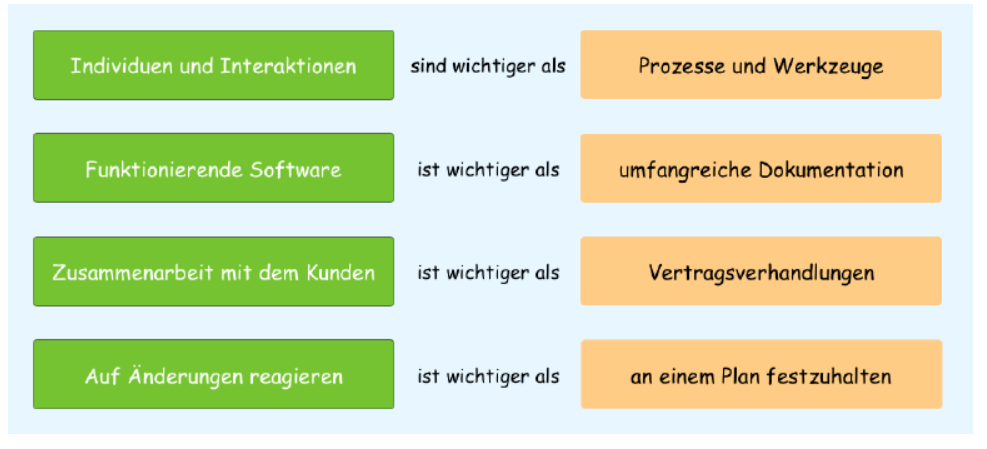
\includegraphics[width=1\textwidth]{figures/daniel/Bild-1.png}
  \caption[]{Scrum Prinzipien verglichen}
  \label{fig:scrum_prinzipien}
\end{figure}

Frei interpretiert wird beim Scrum Framework mehr Wert auf die einzelnen Stakeholder des Projekts gelegt als auf das Projekt selbst. Ebenso werden Bürokratie und umfangreiche Planungen auf ein nötigstes reduziert. Der Ansatz verfolgt dem klaren Ziel, Teilerfolge schnell sichtbar zu machen und den Kunden in frühen Stadien der Arbeit mit in den Projektfortschritt zu integrieren. 

\subsection{Scrum Rollen}
\subsubsection{Product Owner}
Als Product Owner, am ehesten zum klassischen Projektmanagement mit dem Projektleiter vergleichbar, repräsentiert die Bedürfnisse des Endkunden und steht im engen Austausch mit dem Auftraggeber. Seine Aufgabe ist es, die Bedürfnisse des Kunden genau zu verstehen und diese bestmöglich umsetzen zu lassen. Er hat eine klare Vision und vergleicht sprintweise den Fortschritt seines Teams und dem resultierenden Inkrement mit der tatsächlichen Wunschsoftware des Kunden. 

\subsubsection{Scrum Master}
Der Scrum Master, ist in dieser Rolle und Funktion einzigartig im gleichnamigen Framework. Er steht für Teamchemie und Prozessreife, gleichzeitig unterstützt er das Team und den Product Owner und gilt als Problemlöser. Der Zauber in seiner Funktion ist die Eigenständigkeit gegenüber dem eigentlichen Product Owner. Er steht als Mittelsmann in vielerlei Hinsicht. Das Team zu verstehen und die Zusammenarbeit und Kommunikation zu verbessern und fördern ist sein Ziel, nicht der direkte Projekterfolg und die Erfüllung der Kundenbedürfnisse.

\subsubsection{Team}
Das Team ist verglichen mit dem klassischen Projektmanagement eher selbstorganisierter und eigenverantwortlicher in der Erfüllung der vom Projektleiter vorgegebenen Aufgaben. Es wird in regelmäßigen Terminen, später näher erläutert viel über Kommunikation und Austausch koordiniert als stets das stumpfe Erledigen von Aufgaben. Das Einbringen von Ideen und das Kundtun von Problemen und Missständen ist essenziell für den Projekterfolg. 


\subsection{Scrum Artefakte}
\subsubsection{Product Backlog}
Das Product Backlog ist am ehesten mit einem Milestoneplan aus dem klassischen Projektmanagement zu vergleichen. Es stellt eine Liste aller offenen Aufgaben dar und wird vom Product Owner gehegt und gepflegt. Er priorisiert hier sprintweise die zu erledigenden Tätigkeiten nach Wichtigkeit und Dringlichkeit und will für den Kunden den maximal möglichen Umfang rausholen gleichzeitig aber mit enger Abstimmung seines Teams nach deren Möglichkeiten und mit deren technischer Expertise.

\subsubsection{Sprint Backlog}
Der Sprint Backlog ist ein Extrakt aus dem zuvor beschriebenen Product Backlog, reduziert auf die Tätigkeiten eines Sprints. Mit einer Laufzeit von beispielsweise 6 Wochen wird ein gemeinsames Ziel definiert und die dafür zu erfüllenden Aufgaben werden durch den Sprint Backlog als Liste festgehalten. Es erfolgt hier ebenso eine Priorisierung und Zuordnung auf Personen. Die einzelnen Teammitglieder nehmen sich den darin stehenden Aufgaben an und berichtet regelmäßig und eigenständig über den Status der Fertigstellung oder über auftretende Probleme oder benötigte Unterstützung jeglicher Art.

\subsubsection{Product Inkrement}
Das Product Inkrement stellt ein einzelnes Teilergebnis nach einem Sprint dar, auf welches im selbigen hingearbeitet wird. Es soll ein vorzeigbarer und erlebbarer Bestandteil des Gesamtergebnisses sein, welches mit dem Kunden gemeinsam diskutiert wird. Am Produkt Inkrement bekommt das gesamte Team relativ früh und konkret Kundenfeedback über die Zufriedenheit der bisher geleisteten Arbeit. Missverständnisse und Fehler in der Umsetzung sollen sehr schnell aufgezeigt werden.

\subsection{Scrum Events}
\begin{figure}[!htb]
  \centering
  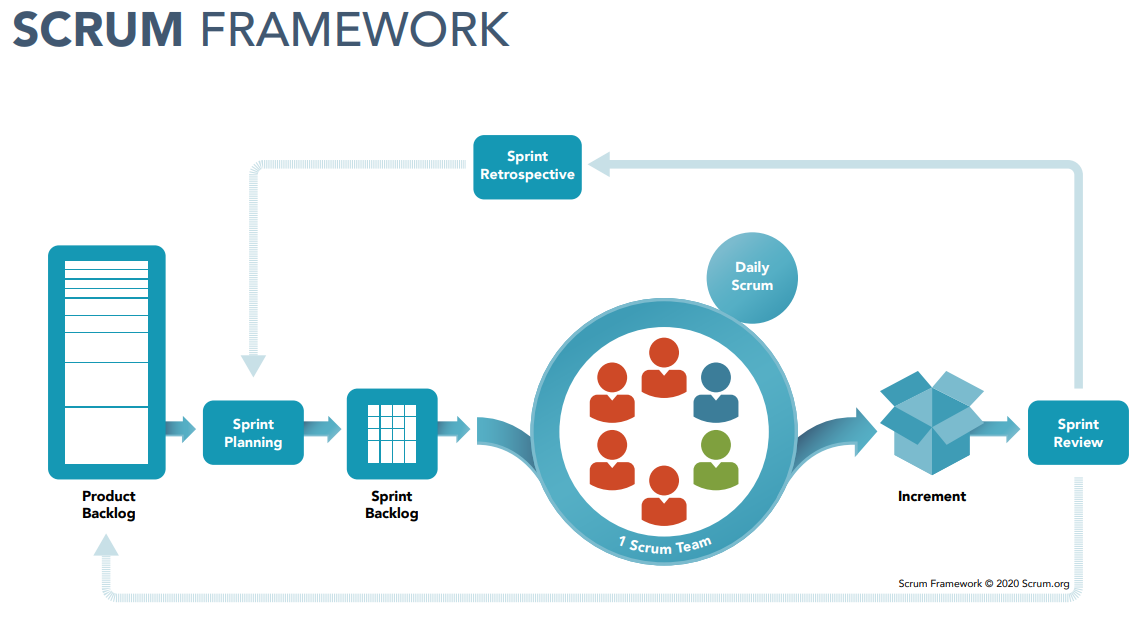
\includegraphics[width=1\textwidth]{figures/daniel/Bild-2.png}
  \caption[]{Scrum-Events im Überblick}
  \label{fig:scrum_events}
\end{figure}

\subsubsection{Sprint}
Der bereits erwähnte Sprint stellt einen Teilabschnitt des Projekts dar. Er besitzt einen eigenen Backlog und wird in der Regel auf 4-8 Wochen terminiert. Innerhalb des Sprints bestimmen weitere Events den Rahmen des Frameworks. Der Sprint selbst steht repräsentativ für das agile Projektmanagement und unterscheidet dich somit klar vom klassischen, oft im Wasserfall ausgelebten Projektmanagement, welches oft nur als Ganzes gesehen wird mit festen Milestones als Einzeletappen.

\subsubsection{Sprint Planning}
Das Sprint Planning stellt den Beginn eines neuen Sprints dar. Hier wird ein Product Inkrement festgelegt, ein gemeinsames Ziel formuliert und deren dafür benötigten Aufgaben definiert. Das Team als Ganzes ist in der Planung involviert. Die Planung selbst erfolgt oftmals über das sogenannte Planning Poker, jedoch kann dieses auch anders praktiziert werden. Jedes einzelne Teammitglied sollte im Austausch mit dem Team selbst und dem Produktowner sowie Scrum Master seinen Arbeitsumfang im Sprint festlegen.



\subsubsection{Weekly Standup}
Das Weekly Standup oftmals auch als Daily Standup praktizierte Event, stellt einen Regeltermin für das gesamte Team dar, in welchem die einzelnen Teammitglieder Ihren aktuellen Arbeitsfortschritt kundtun beziehungsweise kommende Aufgaben und Herausforderungen mit dem Team teilen. Es sollte als kurzes und agiles Event praktiziert werden in welchem auf Probleme und Schwierigkeiten offen und ehrlich mitgeteilt werden. Bei physisch gehaltenen Termin werden die Mitglieder des Termins oft stehend in den Austausch gebracht, online kann dieses zumindest jeder selbst frei entscheiden.

\subsubsection{Sprint Review}
Im Review wird der nun abgeschlossene Sprint begutachtet und der Fortschritt und der Erfolg und Misserfolg objektiv beurteilt. Jedes Mitglied kann seine Aufgaben und Ergebnisse individuell oder als Teil-Team vorstellen und diese gegenüber dem Kunden beziehungsweise dem restlichen Team präsentieren. Es ist darauf zu achten das Event selbst klar von der kommenden Retroperspektive abzugrenzen und persönliche Themen für dieses Event aufzuheben. Der Kunde selbst ist in diesem Event oft involviert.


\subsubsection{Sprint Retrospective}
Die Sprint Retrospective oder auch als Retro bezeichneter Termin, findet gegen Ende des vorangegangenen Sprints statt. Im Gegensatz zum zuvor erwähnten Review werden hier subjektive und zwischenmenschliche Themen miteinander diskutiert. Das Event soll die Möglichkeit schaffen, sich als Team auszutauschen und gegenseitig mit Lob und konstruktiver Kritik zu konfrontieren. Hier ist vor allem der Scrum Master gefragt, eine Atmosphäre zu schaffen und das Team zu ermutigen oft auch unangenehme Themen anzusprechen.

\section{Projektmanagement}
\label{sec:projectmanagement}
% \section{Projectmanagement}

In diesem Abschnitt wird der Bereich des Projektmanagements und der Projektplanung innerhalb des Digital Home Town Teams näher erläutert. Als Hilfsmittel wurde hierfür hauptsächlich die Software JIRA von Atlassian verwendet. Hierbei wird auch auf die einzelnen Tasktypen und deren Bedeutung eingegangen. Des Weiteren wurde ein eigener Arbeitsablauf für das Entwicklerteam definiert. Abschließend wird auf die Sprint-Planung und die spätere Verwendung einer sog. User Story Map eingegangen.

\subsection{JIRA}
JIRA ist ein Tool zur Unterstützung von Projektmanagement-Prozessen, das von vielen Unternehmen und Organisationen genutzt wird. Mit JIRA können Projekte geplant, verwaltet und kontrolliert werden, indem Aufgaben, Meilensteine und Prozesse visualisiert und koordiniert werden. Es bietet auch Funktionen zur Zusammenarbeit und Kommunikation innerhalb des Projektteams sowie zur Nachverfolgung von Fortschritten und Problemen. JIRA kann auch individuell angepasst werden, um den spezifischen Bedürfnissen eines Projekts gerecht zu werden. Im Zuge des Projekts wurden mehrere solcher Anpassungen vorgenommen sowie Teaminterne Regeln festgelegt. Diese sollen im Folgenden Abschnitt näher erläutert werden.

\subsubsection{Tasks}
Die Besonderheit an JIRA ist die Möglichkeit zur Aufteilung von mehreren Arbeiten in sogenannte Tasks. Ein Task hat normalerweise eine eindeutige Identifikationsnummer, eine kurze Beschreibung der Aufgabe, eine Zuweisung an einen Verantwortlichen, einen Status sowie ggf. zusätzliche Informationen wie z.B. Verknüpfungen mit anderen Tasks. 

\begin{figure}[ht!]
    \centering
    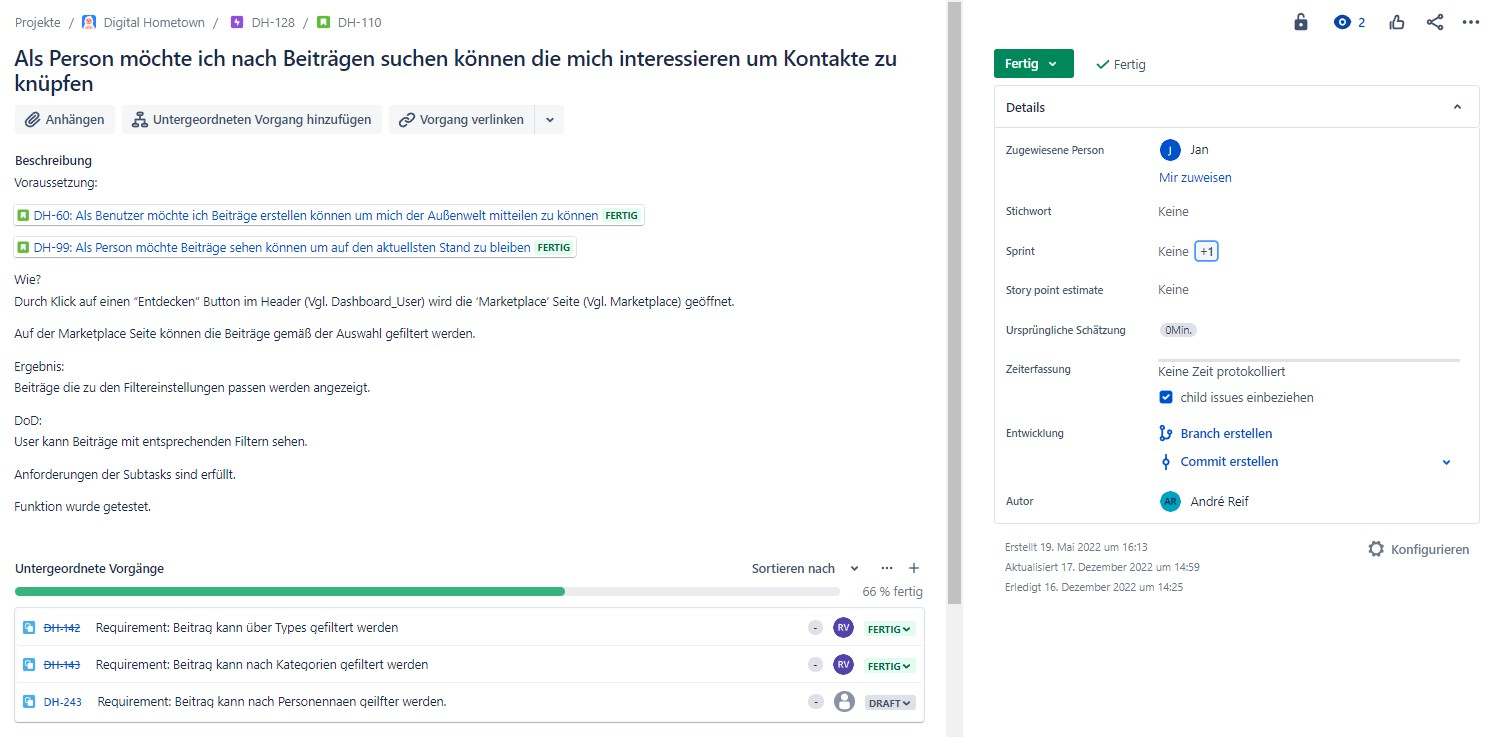
\includegraphics[width=0.6\textwidth]{figures/andre/jiratask.jpg}
    \caption{Beispiel für einen Task im JIRA}
    \label{fig:jiratask}
\end{figure}

Einzelne Tasks können in sog. Epics geclustert werden, um so die Aufgaben und langfristige Planung besser strukturieren zu können. Im Folgenden ist eine Übersicht der Epics innerhalb des Projekts sowie deren Fortschritt zu sehen.

\begin{figure}[ht!]
    \centering
    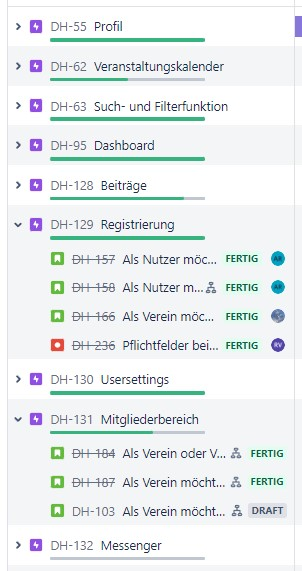
\includegraphics[width=0.6\textwidth]{figures/andre/epicsdesprojekts.jpg}
    \caption{Epic Übersicht des Projekts}
    \label{fig:epicsdesprojekts}
\end{figure}

Für die einzelnen Tasks wurden jeweils 4 verschiedene Typen unterschieden.

\subsubsection*{User-Story}
Eine User Story beschreibt eine neue Nutzeranforderung, also ein Feature, dass umgesetzt werden muss das der Benutzer die entsprechende Tätigkeit ausführen kann. Diese werden per Definition nach dem folgenden Prinzip geschrieben:

Als Nutzer möchte ich \textbf{<Auszuführende Tätigkeit>} um \textbf{<Vorteil oder Intention der ausgeführten Tätigkeit>}.

Eine User Story hat den Folgenden Aufbau:
\begin{itemize}
    \item \textbf{Titel} User Story nach Definition.
    \item \textbf{Wie?} Kurze Beschreibung wie die Funktion umgesetzt werden soll.
    \item \textbf{Ergebnis?} Beschreibung was passiert, wenn die Funktion ausgeführt wird.
    \item \textbf{DoD} Definition of Done, also eine Definition, wann der Task als erledigt gilt.
\end{itemize}

\subsubsection*{Sub-Task}
Sub-Tasks werden in der Regel dazu verwendet, um besonders aufwendige User Stories und Tasks in kleinere Arbeitseinheiten zu unterteilen. Für Digital Home Town wurden die Sub-Tasks verwendet, um Task-spezifische Anforderungen zu dokumentieren und hervorzuheben. 
\subsubsection*{Functional-Task}
Für unterstützende Arbeiten, die nicht direkt mit der Entwicklung der Plattform in Verbindung stehen, wurden sog. Functional Tasks eingeführt. Diese sind in der Regel nicht näher definiert oder Beschrieben und sind Anhand des Titels nachvollziehbar. 

\begin{figure}[ht!]
    \centering
    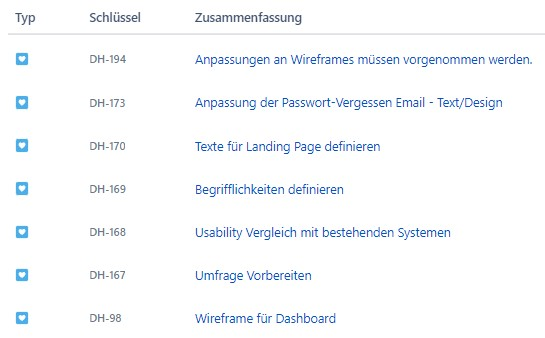
\includegraphics[width=0.6\textwidth]{figures/andre/functionaltasks.jpg}
    \caption{Beispiele für Functional Tasks}
    \label{fig:functionaltasks}
\end{figure}

\subsubsection*{Bug}
Ein Bug stellt einen gefundenen Fehler auf der Plattform da. Dieser spiegelt sowohl einen Fehlerbericht als auch einen neuen Arbeitsauftrag dar. Innerhalb des Entwicklerteams war es üblich, dass zumeist der Verursacher des Bugs auch für dessen Behebung verantwortlich war. Ein Bug durchläuft allerdings denselben Arbeitsablauf wie eine User-Story und nach den gleichen Standards getestet.

\begin{figure}[ht!]
    \centering
    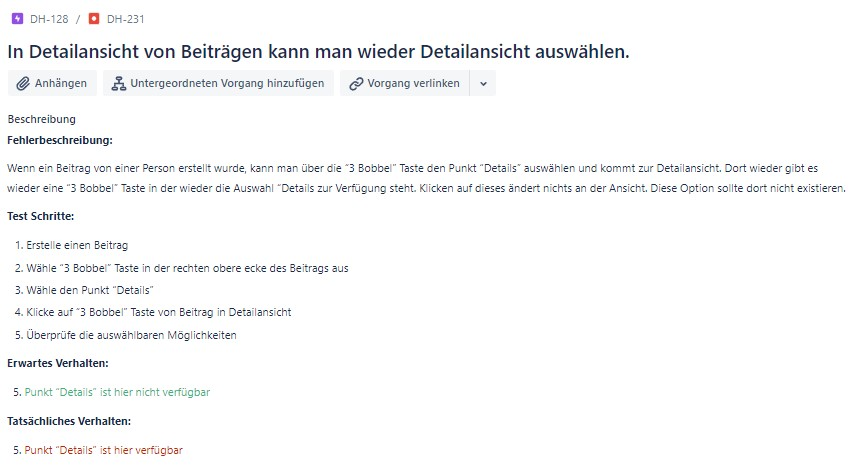
\includegraphics[width=0.6\textwidth]{figures/andre/bugticket.jpg}
    \caption{Beispiel für ein Bug Ticket}
    \label{fig:bugticket}
\end{figure}

Ein Bug besteht in der Regel aus:

\begin{itemize}
    \item \textbf{Titel} Kurze Beschreibung des Fehlers
    \item \textbf{Beschreibung} Detaillierte Beschreibung des Fehlers und des Fehlerhergangs
    \item \textbf{Test Schritte} Schritt-für-Schritt Angaben über den Ablauf des Tests
    \item \textbf{Verhalten} Erwartetes und Tatsächliches Verhalten
\end{itemize}

\subsubsection{Arbeitsablauf}
In der folgenden Abbildung ist der Allgemeine Arbeitsablauf für ein einzelnes JIRA Ticket zu sehen.

\begin{figure}[h!]
    \centering
    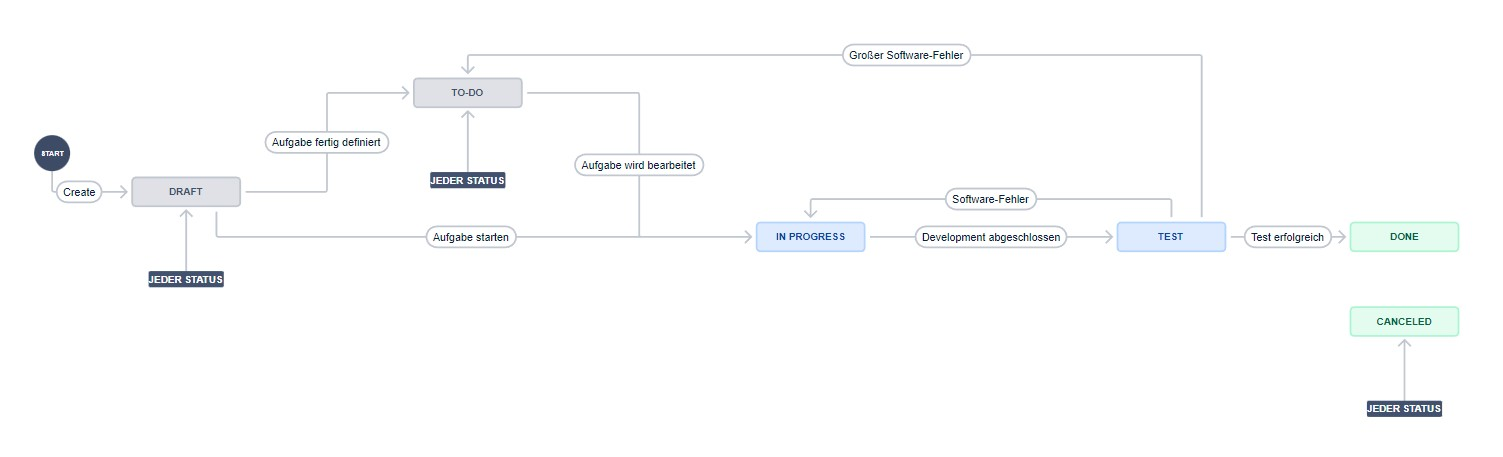
\includegraphics[width=0.6\textwidth]{figures/andre/workflow.jpg}
    \caption{Darstellung des Ablaufs eines einzelnen JIRA Tickets}
    \label{fig:workflow}
\end{figure}

Ein einzelner Task wurde zunächst mit dem Status „Draft“ erstellt. Dies wurde im Allgemeinen so interpretiert, dass das Ticket zwar angelegt wurde, jedoch nicht vom Team so akzeptiert wurde, dass jeder die Aufgabe verstanden hat. Dies wurde bei der Sprint Planung bzw. dem Task Refinement während der Planung Besprochen, ggf. angepasst, und dann festgelegt. 

Nachdem ein Task den Status „ToDo“ erhält, kann dieser in einem Sprint eingeplant und entsprechend bearbeitet werden. Der Status wechselt demnach zu „In Progress“. 

Nach der Bearbeitung wird ein Ticket mit Hilfe des Flags „Test“ zum Testen freigegeben. Das Bedeutet der Code läuft in der Entwicklungsumgebung und kann von einem Tester bearbeitet werden. Ob im Fehlerfall ein Task zurück in den Status „ToDo“ oder „In Progress“ versetzt wurde, lag in der Schwere des Fehlers und im Ermessen des jeweiligen Testers. Falls der Test erfolgreich war, wurde der Task auf den Status „Done“ verschoben und war somit abgearbeitet.

Aufgrund sich ändernder Anforderungen wurde später der „Canceled“ Staus eingeführt, um ggf. bereits begonnene Tasks abbrechen zu können.

Dieser Ablauf gilt in der Regel für jede User Story sowie jeden Bug. Die Stati „Draft“ und „Test“ hatten für Functional Tasks und Sub Tasks jedoch keine tiefergehende Bedeutung und konnten einfach übersprungen werden.

\subsection{Sprint Planning mit JIRA}
Die Sprints wurden in der Regel vorausgeplant. Dabei galt die Regel: der nächste Sprint steht am Ende des aktuellsten Sprints weitestgehend fest, der übernächste Sprint ist zu 50\% geplant. 

Während der Planungsmeetings wurden die geplanten Tasks und Bugs besprochen und auf deren Umsetzbarkeit und Priorität geprüft. Aufgrund der un-terschiedlichen Kenntnisse und Fertigkeiten der Entwickler war es jedoch schwierig den Aufwand einzelner Tasks verallgemeinert für das gesamte Entwicklungsteam einzuschätzen. Zuzüglich dazu mussten Urlaubs- und Abwesenheitszeiten bei der Planung berücksichtigt werden, sodass die definierten Sprint Ziele auch erreicht werden konnten.

\begin{figure}[h!]
    \centering
    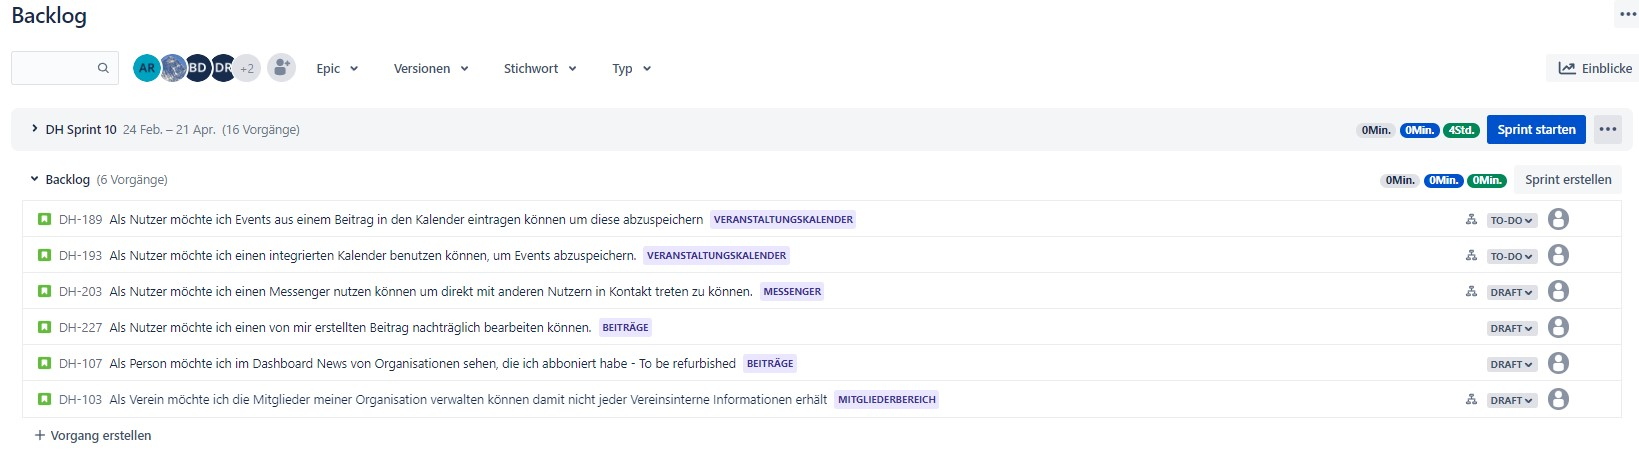
\includegraphics[width=0.6\textwidth]{figures/andre/jirabacklog.jpg}
    \caption{Backlog Funktion im JIRA}
    \label{fig:jirabacklog}
\end{figure}

Zur Planung der Sprints wurde die in der obigen Abbildung zu sehende Backlog Funktion verwendet. Hier sind zum sowohl die nicht geplanten Tasks zu sehen als auch die einem Sprint bereits zugeordnetem Task und können auch bei Bedarf entsprechend umgeplant werden. So war es nicht unüblich, dass nachdem das Sprintziel bereits vor dem Ende des Sprints erreicht wurde, noch offene Bugs oder kleinere Functional Tasks dem Sprint hinzugefügt und abgearbeitet wurden. Zum Sprintende begonnene Arbeitsaufträge wurden grundsätzlich in den nachfolgenden Sprint verschoben und fertiggestellt.

\subsubsection{User Story Map}
Als weiteres Tool zur Projektplanung wurde der Ansatz des sogenannten User Story Mapping verwendet. Per Definition ist eine User Story Map eine Technik zur Visualisierung von Benutzeranforderungen und -funktionen in einer hierarchischen Struktur.

\begin{figure}[h!]
    \centering
    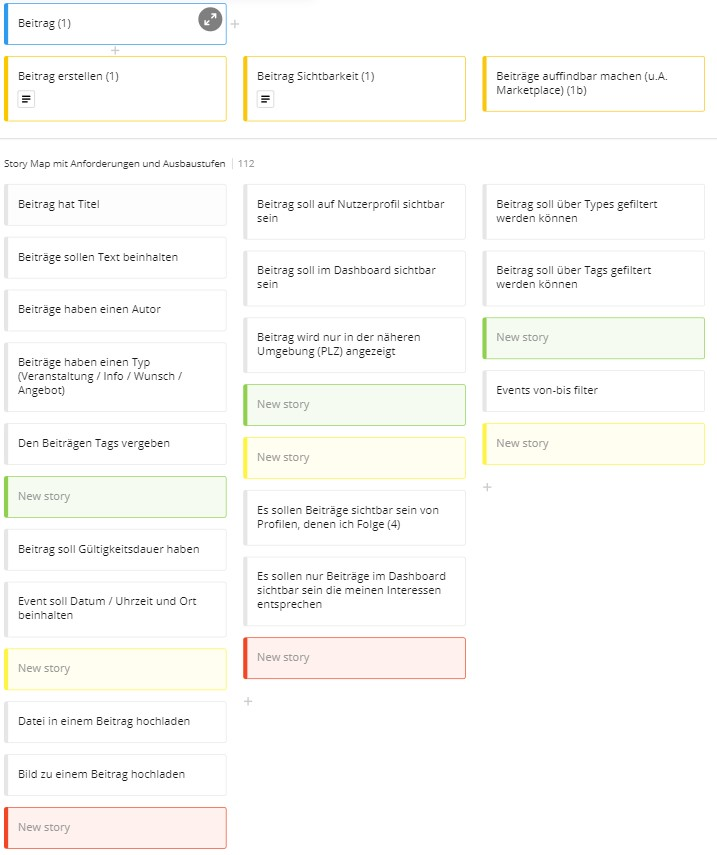
\includegraphics[width=0.6\textwidth]{figures/andre/userstorymap.jpg}
    \caption{Beiträge in der User Story Map}
    \label{fig:userstorymap}
\end{figure}

In der obigen Abbildung ist die User Story Map für einige Features der Beiträge zu finden. So gibt es zur User Story „Als Nutzer möchte ich einen Beitrag erstellen können um mich der Community mitteilen zu können“ verschiedene Anforderungen. Diese stehen unterhalb des jeweils gelben Blocks. 

Die Anforderungen jeweils wurden dann in 3 Iterationsstufen Priorisiert:

\begin{itemize}
    \item \textbf{Bis Grün} Minimum viable product, also die Minimalanforderungen die Umgesetzt werden sollen
    \item \textbf{Bis Gelb} Nice-to-Have, Anforderungen die umgesetzt werden sollen, aber nicht hoch Priorisiert werden
    \item \textbf{Bis Rot} Wird implementiert falls genügend Zeit dafür da ist
\end{itemize}

Aus dieser Map wurden dann die einzelnen User Story Tasks im JIRA angelegt und entsprechend in den Sprints verplant.

\section{Sprintübersicht}
\label{sec:sprintoverview}
\input{content/03_process/03_Sprintübersicht}

\chapter{Technologien}
\label{ch:technical}

Für die Entwicklung eines Softwaresystems ist insbesondere bei der Implementierung entscheidend, welche Technologien verwendet werden.
Aus diesem Grund widmet sich diese Kapitel werden die technischen Aspekte der Plattform beschrieben.
Dabei werden die Technologien und Frameworks vorgestellt, die für die Entwicklung der Plattform verwendet wurden.

Die Plattform wurde mit den folgenden Technologien und Frameworks entwickelt:
\begin{itemize}
  \item \textbf{TypeScript} als Programmiersprache
  \item \textbf{React} als Frontend-Framework
  \item \textbf{\gls{mui}} als UI-Framework
  \item \textbf{Firebase} als Backend as a Service (\gls{baas})Plattform
  \item \textbf{Vercel} als Hosting-Plattform
  \item \textbf{Github} als Versionsverwaltungs-Plattform
  \item \textbf{Jira} als Projektmanagement-Plattform
\end{itemize}

Diese werden im Folgenden kurz vorgestellt.

\section{Grundlage für Technologieentscheidung}
\label{sec:technicalDecision}

Die einzige aus der Aufgabenstellung ersichtliche Vorgabe ist, dass das Softwareprodukt „Digital Hometown“ eine Plattform für den Austausch bieten soll.
Die Wahl der Technologie ist uns hierbei offengelassen.
Was daraus jedoch hervorgeht ist, dass es sich um eine für möglichst viele Nutzer verwendbare Web- oder Mobilanwendung handeln soll.
Insbesondere bei der Wahl einer Webanwendung, die dem Nutzer jeglichen Installationsaufwand erspart, ist die Hemmschwelle sehr gering, ein Softwareprodukt auszuprobieren.

Da, wie beschrieben, für eine solche Plattform des sozialen Austauschs eine ausreichend große Nutzerzahl entscheidend ist, fiel die Entscheidung schnell auf eine Webanwendung.
Obwohl beim aktuellen Stand der Plattform „Digital Dahoam“ nicht in erster Linie auf die Benutzbarkeit auf mobilen Endgeräten gelegt wurde, sei an dieser Stelle erwähnt, dass sich Webanwendungen mit etwas mehr Aufwand sehr gut auch für mobile Geräte wie Smartphones oder Tablets entwickeln lassen.
Der Fachbegriff hierfür ist die Umsetzung einer „Progressive Web-App“.

\section{TypeScript}
\label{sec:typescript}

TypeScript ist eine Erweiterung von Javascript, die statische Typisierung und Klassen hinzufügt.
Dadurch wird die Entwicklung von Software vereinfacht, da die Typisierung die Lesbarkeit des Codes verbessert und die Klassen die Wiederverwendbarkeit von Code ermöglichen.
Die Programmiersprache wird von Microsoft entwickelt und ist Open Source.\footnote{Vgl. TypeScript 2022 \cite{typescript2022}}

\subsection{Einsatz im Projekt}
\label{sub:typescriptUsage}

TypeScript wurde im Projekt verwendet, um die Entwicklung der Plattform zu vereinfachen. Der komplette Code der Website wurde mit TypeScript, HTML und CSS geschrieben, wobei TypeScript hierbei die Hauptrolle spielt.

\subsection{Grund für Technologieentscheidung}
\label{sub:typescriptReason}

Da TypeScript in großen Teilen der Javawelt inzwischen als de facto Standard ist um vor allem große Anwendungen sicher und effizient zu entwickeln, wurde diese Technologie für die Entwicklung der Plattform verwendet.
React (\ref{sec:react}), das größte Frontend-Framework der Welt, wird inzwischen auch in TypeScript entwickelt.\footnote{Vgl. TypeScript 2023 \cite{typescript2023}}

\section{React}
\label{sec:react}

React ist ein Open-Source Frontend-Framework, das von Facebook entwickelt wird.
Es ermöglicht die Entwicklung von Benutzeroberflächen für Webanwendungen.
Dabei wird die Benutzeroberfläche in einzelne Komponenten aufgeteilt, die unabhängig voneinander entwickelt werden können.
Diese Komponenten werden in einer \texttt{.\gls{jsx}} Datei definiert, die eine Kombination aus Javascript und HTML ist.
Die Komponenten werden in einer \gls{react} Anwendung in einer \texttt{.\gls{jsx}} Datei eingebunden.
In einer neueren Version, ist es auch möglich mit TypeScript zu arbeiten.
 Die neue Dateierweiterung für diese TypeScript ist \texttt{.\gls{tsx}}.
Diese Dateien werden dann in eine Javascript Datei kompiliert, die von einem Browser ausgeführt werden kann.\footnote{Vgl. React 2022 \cite{react2022}}

\subsection{Allgemeines in Bezug auf die Implementierung mit React}
\label{sub:reactGeneral}

React basiert auf dem Model-View-Controller Design Pattern. Der Browser Document Object Model (DOM) fungiert dabei als die View-Komponente. Die Model-Komponente, ist der Virtual DOM, das vom Controller (React) manipuliert wird.

\subsubsection{Einrichten und Starten der React-Anwendung}
\label{sub:reactSetup}

Für die Entwicklung von React-Anwendungen eignen sich alle moderne Entwicklungsumgebungen. Im Projektteam wurde sich auf den weitverbreiteten Texteditor „Visual Studio Code“ geeinigt. Neben einer Entwicklungsumgebung wird Node.js benötigt, um Javscript-Code auf der Entwicklungsmaschine ausführen zu können. Die notwendigen Abhängigkeiten werden mit dem Paketmanager „yarn“ installiert.
Mit dem in der Datei package.json definierten Alias yarn dev startet der lokale Node.js Entwicklungsserver automatisch, nachdem alle benötigten Pakete installiert wurden.
Handelt es sich um eine lauffähige Version, wird automatisch im Browser die Startansicht der entwickelten React-Anwendung geöffnet.

\subsubsection{React Components}
\label{sub:reactComponents}

React besteht aus Komponenten, die automatisch neu gerendert werden, wenn sich die Parameter der Komponente ändern.
Komponenten können als Functional- bzw. als Class-Komponenten implementiert werden.
Während die Verwendung von Class-Komponenten in älteren React-Versionen üblich war, wird in den aktuellen Versionen meist die funktionelle Implementierung verwendet.

\begin{lstlisting}[language=JavaScript, label=reactComponent, title={Beispiel einer React-Komponente}]
  function Component(props: {name: string}) {
    return <div>Hallo {props.name}!</div>
  }
\end{lstlisting}

\subsubsection{React Hooks}
\label{sub:reactHooks}
Die Komponenten bilden die Basis jeder React-Anwendung. Durch die React-Hooks wird es einer Komponente ermöglicht, dynamische Bestandteile und einen Zustand zu besitzen. Es gibt mehrere Hooks für verschiedene Anwendungsfälle und es lassen sich auch eigene Hooks definieren. Eines der wichtigsten React-Hooks ist useState. Durch useState wird es ermöglicht, eine Variable über ein oder mehrere Komponenten hinweg zu benutzen und manipulieren. Die Verwendung eines useState Hooks wird in Code 2 gezeigt. Hier wird auch ein weiterer wichtiger Hook aufgeführt. Der useEffect Hook ermöglicht es, auf die Änderung eines Zustands zu reagieren.

\begin{lstlisting}[language=JavaScript, label=reactComponentHooks, title={Beispiel einer React-Komponente mit Hooks}]
function Component() {
  // count ist der aktuelle Wert
  // setCount ist die Funktion, um den Wert zu ändern
  const [count, setCount] = React.useState<number>(0)

  React.useEffect(() => {
    // wird ausgeführt, wenn count sich ändert
    console.log("count changed")
  }, [count])

  return (
    <div>
      <p>{count} mal geklickt.</p>
      <button onClick={() => setCount(count + 1)}></button>
      Button
    </div>
  )
}
\end{lstlisting}

Es lassen sich beliebig viele Komponenten verschachteln. Das Durchreichen der Parameter wird bei größeren Projekten sehr aufwändig – insbesondere in Bezug auf die Wartbarkeit. Um dies zu entschärfen, gibt es weitere Konzepte wie der React Context, der im Folgenden beschrieben wird.

\subsubsection{React Context}
\label{sub:reactContext}

Der React Context ermöglicht es einen Zustand über mehrere Komponenten hinweg zu benutzen, ohne ihn mittels Parameter an alle Unterkomponenten durchzureichen. Man kann den React Context mit einer globalen Variable vergleichen.
Ein typischer Anwendungsfall für den React Context ist das Verwenden von Authentifizierungsdaten wie der Name über die gesamte Anwendung hinweg.

\subsection{Einsatz im Projekt}
\label{sub:reactUsage}

React wurde verwendet, um die gesamte Website aufzubauen.
Sie bildet alles ab, was der Benutzer sieht und mit der Plattform interagiert.

\subsection{Grund für Technologieentscheidung}
\label{sub:reactReason}

React wurde für die Entwicklung der Plattform verwendet, da es das meistgenutzte Frontend-Framework der Welt ist.
Außerdem gab es ein großes Interesse der verschiedenen Entwickler, sich in dieses Framework einzuarbeiten.

\begin{figure}[ht!]
  \begin{centering}
    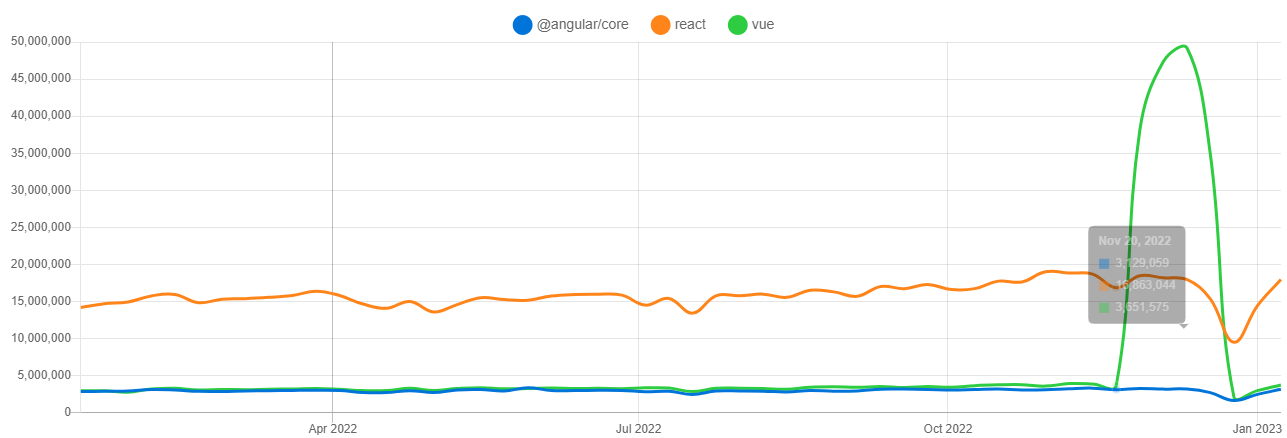
\includegraphics[width=.75\textwidth]{figures/technical/frontendFrameworks.png}
    \caption{Vergleich Downloadzahlen verschiedener Frontend Frameworks \cite{npm2023}}
    \label{fig:downloadFrontendFrameworks}
  \end{centering}
\end{figure}

\section{Material-UI}
\label{sec:material-ui}

Material-UI (kurz \gls{mui}) ist eine Bibliothek, die es ermöglicht, Komponenten aus dem Material Design zu verwenden.
Diese Komponenten sind konfigurierbar und können so an die eigenen Bedürfnisse angepasst werden.
Trotzdem entsprechen Sie alle einer einheitlichen Designsprache, die von Google entwickelt wurde. \footnote{Vgl. Google 2021 \cite{google2021}}

MUI bietet Komponenten für folgende Bereiche an:

\begin{itemize}
  \item \textbf{Navigation} – Komponenten für die Navigation.
  \item \textbf{Inputs} – Komponenten für die Eingabe von Daten.
  \item \textbf{Layout} – Komponenten für das Layout der Website.
  \item \textbf{Data Display} – Komponenten für die Anzeige von Daten.
  \item \textbf{Feedback} – Komponenten für die Rückmeldung an den Benutzer.
  \item \textbf{Surfaces} – Komponenten für Oberflächen.
  \item \textbf{Utils} – Komponenten für die Unterstützung.
\end{itemize}

Diese Bibliothek wird von Material-UI SAS. entwickelt und ist Open-Source auf Github verfügbar.
MUI bietet eine direkte Integration mit React. \footnote{Vgl. Material-UI 2022 \cite{mui2022}}

\subsection{Einsatz im Projekt}
\label{sub:material-uiUsage}

Da React nur sehr rudimentäre Komponenten für die Benutzeroberfläche bereitstellt, wurde MUI verwendet, um die Benutzeroberfläche zu gestalten.
Es bietet eine große Auswahl an Komponenten, die direkt in React verwendet werden können.

\subsection{Grund für Technologieentscheidung}
\label{sub:material-uiReason}

MUI vereinfachte die Gestaltung der Benutzeroberfläche, da es eine große Auswahl an Komponenten bietet, die direkt in React verwendet werden können.
Aus diesem Grund konnten die Entwickler schnell mit der Gestaltung der Benutzeroberfläche beginnen.

\section{Firebase}
\label{sec:firebase}

Firebase ist eine \gls{baas} Plattform, die die Bereitstellung von Backend-Funktionalität ermöglicht inklusive Datenbank, Authentifizierung, Datei-Upload, etc.
Dabei wird die Funktionalität in einzelne Module aufgeteilt, die unabhängig voneinander verwendet werden können.
Die Plattform wird von Google entwickelt\footnote{Vgl. Firebase 2022 \cite{firebase2022}} und besteht aus mehreren Komponenten, die nun kurz vorgestellt werden.

\subsection{Firebase Authentication}
\label{sub:firebase-authentication}

Firebase Authentication ist ein Modul von Firebase, das die Authentifizierung von Nutzern ermöglicht.
Dabei werden verschiedene Authentifizierungsmethoden unterstützt, wie z. B. E-Mail und Passwort, Google, Facebook, etc.
Außerdem ist es möglich eigene Authentifizierungsmethoden zu implementieren, sowie Nutzer über Telefonnummern zu authentifizieren.
Dabei können Nutzer auch in mehreren Geräten gleichzeitig eingeloggt sein.

Bis auf die Authentifizierungsmethode über Telefonnummern, die nur in den USA verfügbar ist, werden alle Authentifizierungsmethoden kostenlos angeboten. \footnote{Vgl. Firebase Authentication 2022 \cite{authentication2022}}

\subsection{Firebase Realtime Database}
\label{sub:firebase-realtime-database}

Firebase Realtime Database ist ein Modul von Firebase, das die Bereitstellung einer Datenbank ermöglicht.
Diese Datenbank ist eine NoSQL Datenbank, ähnlich wie MongoDB.
Hier werden die Daten nicht relational in Dokumenten gespeichert, sondern in einer Baumstruktur.
Updates in der Datenbank werden in Echtzeit an alle Nutzer gesendet, die sich mit der Datenbank verbinden.\footnote{Vgl. Firebase Realtime Database 2022 \cite{realtimedatabase2022}}

\subsection{Firebase Cloud Firestore}
\label{sub:firebase-cloud-firestore}

Firebase Cloud Firestore ist ein Modul von Firebase, das die Bereitstellung einer Datenbank ermöglicht.
Dabei wird die Datenbank in einzelne Dokumente aufgeteilt, die in einer Baumstruktur organisiert sind.
Firestore ist die Weiterentwicklung der Realtime Database und bietet einige Vorteile gegenüber dieser.
So ist die Datenbank in mehrere Regionen aufgeteilt, was die Verfügbarkeit erhöht.
Außerdem ist es möglich, die Datenbank in mehrere Projekte aufzuteilen, was die Sicherheit erhöht.
Abfragen in der Datenbank können mit Indexen optimiert werden, was die Performance verbessert. \footnote{Vgl. Firebase Cloud Firestore 2022 \cite{firestore2022}}

\subsection{Firebase Storage}
\label{sub:firebase-storage}

Firebase Storage ist ein Modul von Firebase, das die Bereitstellung von Datei-Upload ermöglicht.
Dabei können Dateien in einem Bucket gespeichert werden, das in einzelne Ordner aufgeteilt ist.
Der Datei-Upload kann über die Firebase Konsole oder über die Firebase SDK’s erfolgen.
Diese Funktion ist vergleichbar mit AWS S3 Buckets.\footnote{Vgl. Firebase Storage 2022 \cite{cloudstorage2022}}

\subsection{Einsatz im Projekt}
\label{sub:firebase-use}
Firebase wurde im Projekt für die Bereitstellung der Datenbank und der Authentifizierung verwendet.
Außerdem speichert es die Bilder, die von den Nutzern hochgeladen werden.


\subsection{Grund für Technologieentscheidung}
\label{sub:firebase-reason}
Durch Firebase konnte die Entwicklung der Backend-Funktionalität beschleunigt werden, da die Entwickler sich nicht um die Bereitstellung dieser Funktionalität kümmern mussten.

\section{Github}
\label{sec:github}

Github ist eine Plattform, die es ermöglicht, Softwareprojekte zu verwalten.
Diese Plattform wird von Github Inc. entwickelt. Github bietet eine direkte Integration mit Git.
Die wichtigsten Funktionen von Github sind in Tabelle \ref{tab:github} aufgeführt.\footnote{Vgl. Github 2022 \cite{github2022}}

\begin{table}[ht]
  \begin{tabularx}{\textwidth}{|l|X|}
  \hline
  \textbf{Funktion} & \textbf{Beschreibung} \\ \hline
  Versionsverwaltung & Github bietet Versionsverwaltung auf Grundlage von Git an. \\ \hline
  Projektmanagement & Anforderungen können als Issues angelegt und verwaltet werden. \\ \hline
  Dokumentation & Mithilfe von Markdown Wikis. \\ \hline
  Teamarbeit & In Form von Kommentaren, Reviews, etc. \\ \hline
  Hosting & Bereitstellung statischer Seiten. \\ \hline
  \gls{ci}/\gls{cd} & Automatisierte Tests und Deployment. \\ \hline
  \end{tabularx}
  \caption{Funktionen von Github}
  \label{tab:github}
\end{table}

\subsection{Einsatz im Projekt}
\label{sub:github-use}

Github wurde im Projekt für die Versionsverwaltung und \gls{ci} verwendet.
Die Versionsverwaltung wurde durch die Integration mit Git ermöglicht.
Außerdem wurden Github Actions benutzt, welches automatisierte Tests und andere Sanity-Checks ermöglicht.

\subsection{Grund für Technologieentscheidung}
\label{sub:github-reason}

Github wurde im Projekt eingesetzt, da es eine gute Integration mit Git bietet und somit die Versionsverwaltung vereinfacht.
Außerdem wurde durch die verfügbare \gls{ci} Funktionalität die Qualität des Codes verbessert und stetig getestet werden.
Die Entwicklungsgeschwindigkeit wurde dadurch vereinfacht.

\section{Vercel}
\label{sec:vercel}

Vercel ist eine Hosting-Plattform, die es ermöglicht, statische Webseiten zu hosten.
Diese Plattform wird von Vercel Inc. entwickelt.
Vercel bietet eine direkte zu \ref{sec:github} und erstellt neue Deployments und Builds, sobald ein neuer Commit in Github verfügbar ist.
Dies funktioniert auch mit mehreren Branches und Pull Requests. Jedes Deployment wird mit einer eigenen URL versehen, sodass mehrere Versionen der gleichen Webseite gleichzeitig verfügbar sind.
So können Pull Requests getestet werden, bevor sie in den Master Branch gemerged werden.\footnote{Vgl. Vercel 2022 \cite{vercel2022}}

\subsection{Einsatz im Projekt}
\label{sub:vercel-use}

Vercel wurde im Projekt für die Bereitstellung der Webanwendung verwendet.
Sobald bei Github ein neuer Commit verfügbar ist, wird automatisch ein neues Deployment erstellt.
Dies geschah für den main-Branch auf der Domain \url{https://dahoam.roser.dev} und für den dev-Branch auf der Domain \url{https://dev.dahoam.roser.dev}.
Jeder andere Branch bekam sein eigenes Deployment auf einer eigenen Domain, welche von Vercel erstellt wurde.

\subsection{Grund für Technologieentscheidung}
\label{sub:vercel-reason}

Vercel wurde verwendet, um die Bereitstellung der Webanwendung zu vereinfachen.
Nach Errichtung des Github Repositories und initialer Projekterstellung wurde die Integration mit Vercel in wenigen Klicks aktiviert und hostet seitdem kostenlos die Webanwendung.

\clearpage
\section{Jira}
\label{sec:jira}

Jira ist eine Plattform, die es ermöglicht, Softwareprojekte zu verwalten.
Diese Plattform wird von Atlassian entwickelt.

Die wichtigsten Funktionen von Jira sind in Tabelle \ref{tab:jira} aufgeführt.\footnote{Vgl. Atlassian 2023 \cite{attlassian2023}}

\begin{table}[ht]
  \begin{tabularx}{\textwidth}{|l|X|}
  \hline
  \textbf{Funktion} & \textbf{Beschreibung} \\ \hline
  Projektmanagement & Anforderungen können als Issues angelegt und verwaltet werden. \\ \hline
  Dokumentation & Mithilfe von Markdown Wikis. \\ \hline
  Teamarbeit & In Form von Kommentaren, Reviews, etc. \\ \hline
  \end{tabularx}
  \caption{Funktionen von Jira}
  \label{tab:jira}
\end{table}

\subsection{Einsatz im Projekt}
\label{sub:jira-use}

In Jira wurden die einzelnen User Stories verwaltet und bearbeitet, sowie in Sprints eingeplant.
Durch ein Kanbanboard wurden die einzelnen User Stories in den einzelnen Sprints angezeigt.
Jira bietet eine direkte Integration mit Github.

\subsection{Grund für Technologieentscheidung}
\label{sub:jira-reason}

Jira wurde verwendet, um die Verwaltung der User Stories zu vereinfachen.
Durch die direkte Integration mit Github wurden die einzelnen User Stories mit den dazugehörigen Commits verknüpft.
Dadurch konnte die Entwicklung der einzelnen User Stories nachvollzogen werden.
Außerdem ist es ein sehr simples Tool, welches für die Verwaltung von User Stories sehr gut geeignet ist.

\chapter{Architektur}
\label{ch:architecture}

Auf Grundlage der Technologie Entscheidungen wurde folgende Architektur für das Projekt entwickelt.
Diese ist in folgender Abbildung dargestellt und wird in diesem Kapitel noch genauer erklärt:

\begin{figure}[ht!]
  \begin{centering}
    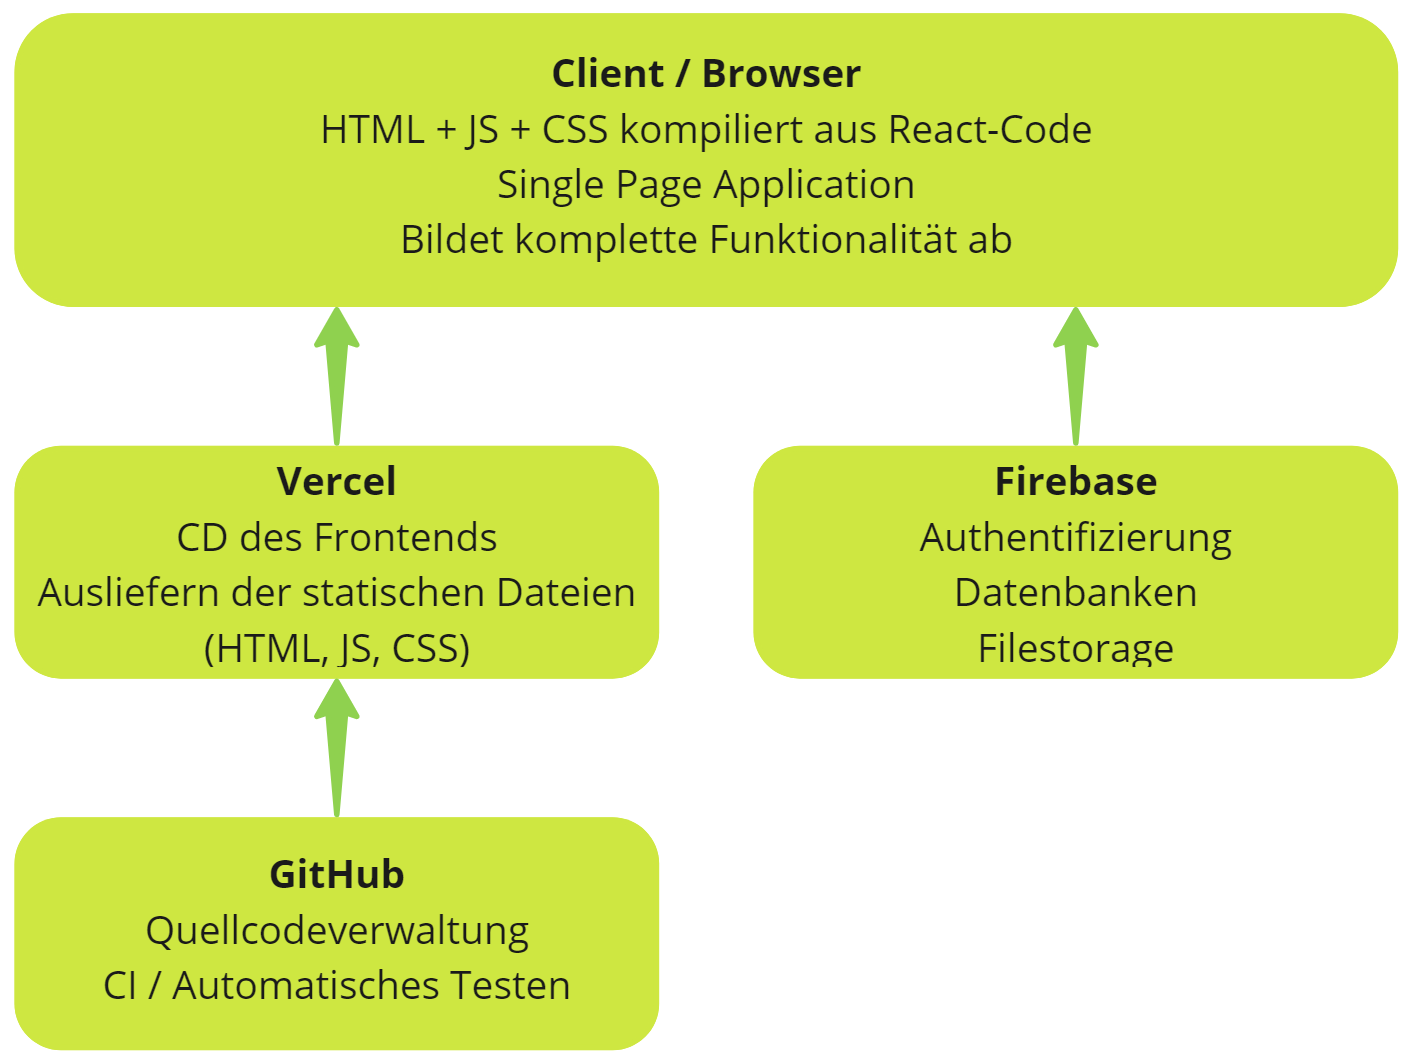
\includegraphics[width=.75\textwidth]{figures/architecture/architecture.png}
    \caption{Übersicht der technischen Softwarearchitektur}
    \label{fig:technicalArchitecture}
  \end{centering}
\end{figure}

Das Frontend wird in React entwickelt. Dieses enthält die Single Page Application (SPA) für die Benutzeroberfläche. Die gesamte Funktionalität wird in diesem Frontend implementiert.
Um im Team bei der Entwicklung effizient zusammenzuarbeiten, wir als Quellcodeverwaltungstool Git bzw. Github verwendet.
Wird eine Änderung am Quellcode veröffentlicht, werden automatisch die CI / CD Prozesse gestartet.
Sind die Tests erfolgreich, wird die neue Version über Vercel gehostet.

Wird der entsprechende Internetlink im Browser aufgerufen, erhält der anfragende Client (Browser) die statischen Dateien für die Benutzeroberfläche.
Der Browser führt das darin enthaltene Javascript aus, das ein dynamisches Laden der Inhalte der Datenbank (Firebase) ermöglicht.

\chapter{Implementierung}
\label{ch:implementation}

In diesem Kapitel wird die Implementierung der Anwendung beschrieben.
Hierbei wird exemplarisch auf zwei wichtige Funktionen der Anwendung eingegangen.
Diese sind die Verwaltung des Benutzerprofils und die Erstellung und Anzeige von Beiträgen.

Da der komplette Code und viele Screenshots den Rahmen dieses Kapitels sprengen würden, wird in den einzelnen Kapiteln nur ein Auszug gezeigt.
Den kompletten Code findet man direkt im Github Repository unter \url{https://github.com/Jonasdero/digital-hometown-frontend}.

\section{Profil}
\label{sec:profile}

Die Profile eines Nutzers sind in der Anwendung sehr wichtig.
Jeder Nutzer verwaltet sein eigenes Profil, welches er mit anderen Nutzern teilt.
Dazu gehören Informationen wie Name, E-Mail-Adresse, Geburtsdatum, Geschlecht und ein Profilbild.
Damit andere Nutzer die Informationen des Profils sehen können, muss das Profil öffentlich sein.
Zudem sollen Benutzer der Anwendung durch Interessen, Profilbilder und persönliche Beschreibungen voneinander unterscheidbar sein und sich so besser vernetzen können.
Um sich mit anderen Nutzern zu verbinden, ist es wichtig, dass diese Informationen in der Anwendung gespeichert werden.

Außerdem soll die soziale Interaktion zwischen Nutzer ermöglicht werden.
Dazu gehören Funktionen wie das Folgen von anderen Nutzern oder auch das Schreiben von Nachrichten zwischen zwei Nutzern oder in Gruppen.
Dies soll direkt vom Profil eines Nutzers aus möglich sein.

\begin{figure}[ht!]
  \begin{centering}
    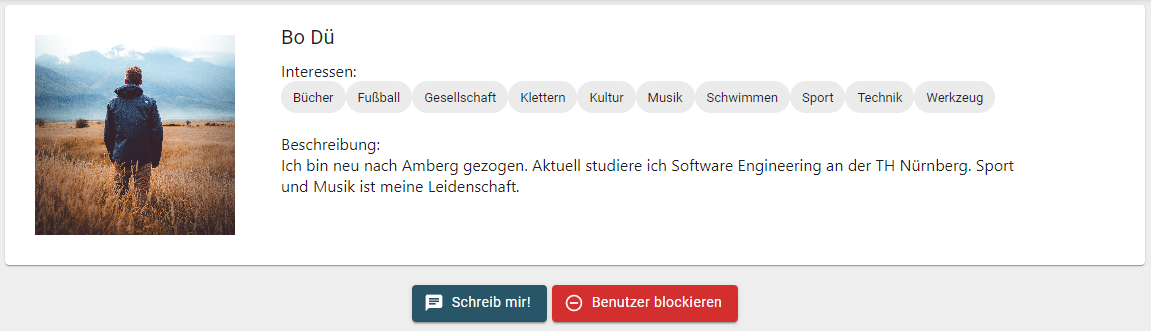
\includegraphics[width=1\textwidth]{figures/implementation/profile-header.png}
    \caption{Übersicht eines Benutzerprofils}
    \label{fig:userProfileHeader}
  \end{centering}
\end{figure}

Hier sieht man die verschiedenen Informationen, die ein Nutzer in seinem Profil angeben kann.
In den nächsten Seiten wird die Implementierung dieser Funktionen beschrieben.
Diese wird aufgeteilt in die verschiedenen Bereiche: \textit{Anmeldung \& Registrierung}, \textit{persönliches Accountmanagement}, \textit{Profilseite \& Profilbilder} und \textit{blockierte Nutzer}.

\subsection{Anmeldung \& Registrierung}
\label{sec:login}

Den Nutzern wird die Möglichkeit gegeben, sich mit einer E-Mail-Adresse und einem Passwort anzumelden oder eine direkte Anmeldung über OAuth mit Google zu nutzen.
Dies wird beides durch die Firebase Authentication API ermöglicht.

Sobald ein Nutzer sich registriert hat, wird von Firebase intern ein Benutzerprofil erstellt, welches wichtige Nutzermetadaten und Authentifizierungsinformationen enthält.
Außerdem wird bei der Anmeldung über Google das Profilbild mit in Firebase gespeichert.
Die Anmeldemaske sieht wie folgt aus:

\begin{figure}[ht!]
  \begin{centering}
    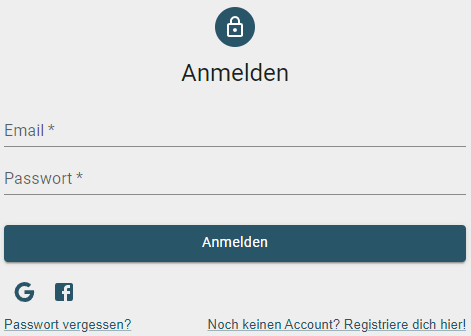
\includegraphics[width=.75\textwidth]{figures/implementation/anmeldemaske.png}
    \caption{Anmeldemaske}
    \label{fig:login}
  \end{centering}
\end{figure}

Um diese Daten in der Anwendung zu speichern, wird ein eigener Benutzerdatensatz angelegt, sobald ein Nutzer registriert wurde und Daten aus dem internen Benutzerprofil von Firebase mit übertragen.
Hierbei wird unterschieden, ob der aktuelle Benutzer ein normaler Nutzer oder ein Verein ist.
Diese werden in unterschiedlichen „Collections“ gespeichert.
Bei der Anmeldung wird dann geprüft, welchen Typ der Benutzer hat und die Daten entsprechend geladen.
Dadurch kann mit einer Datenstruktur gearbeitet werden, die für beide Typen geeignet ist.
Andere Ansichten basieren dann häufig auf der Unterscheidung zwischen Nutzern und Vereinen.
Die Struktur des Datensatzes kann man in Abbildung \ref{fig:firestoreUser} sehen.

\clearpage

\subsection{Persönliches Accountmanagement}
\label{sec:accountmanagement}

Um die Daten des Benutzerprofils zu verwalten, gibt es eine Seite, auf der der Nutzer seine persönlichen Daten ändern kann.
Diese werden dann in der Anwendung aktualisiert und in der Datenbank gespeichert. Er hat hier die Möglichkeit seinen Namen, seine E-Mail, sein Geburtsdatum und seine Postleitzahl zu ändern.
Hier kann außerdem der komplette Account gelöscht werden, um die Daten des Nutzers zu löschen.

\begin{figure}[ht!]
  \begin{centering}
    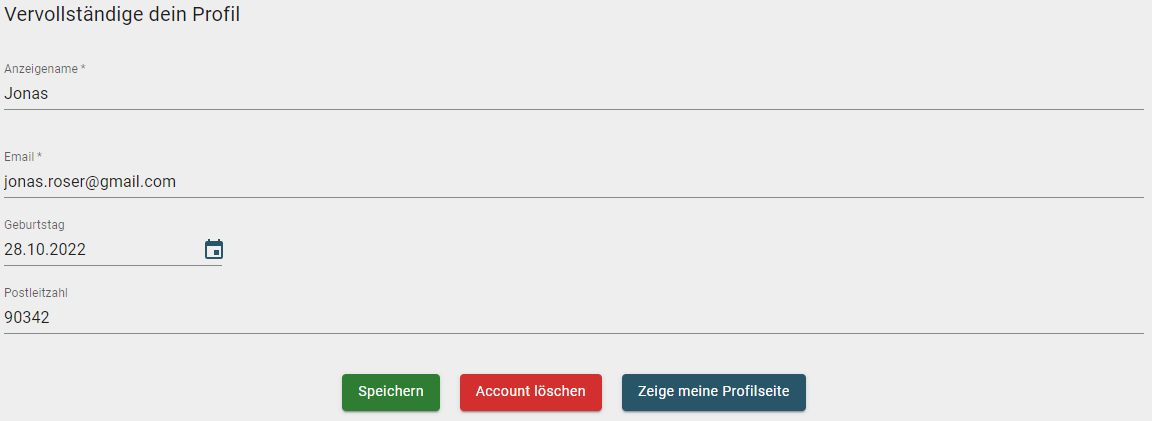
\includegraphics[width=1\textwidth]{figures/implementation/userSettings.png}
    \caption{Benutzereinstellungen}
    \label{fig:userSettings}
  \end{centering}
\end{figure}

\subsection{Profilseite \& Profilbilder}
\label{sec:profilepictures}

Auf der Profilseite des Nutzers kann er seine persönlichen Daten einsehen und bearbeiten. Hier können Interessen und eine Beschreibung hinzugefügt werden.
Außerdem kann er sein Profilbild ändern, indem er auf das Profilbild oder auf den Knopf mit der Kamera klickt.
Dies wird dann im Firebase Storage gespeichert und in der Datenbank verlinkt.

Das Ganze ist so aufgebaut, dass Nutzer zwischen einer Vorschau, also der Sicht, die auch andere Nutzer von seinem Profil sehen und der Bearbeitungssicht unterscheiden können.

\begin{figure}[ht!]
  \begin{centering}
    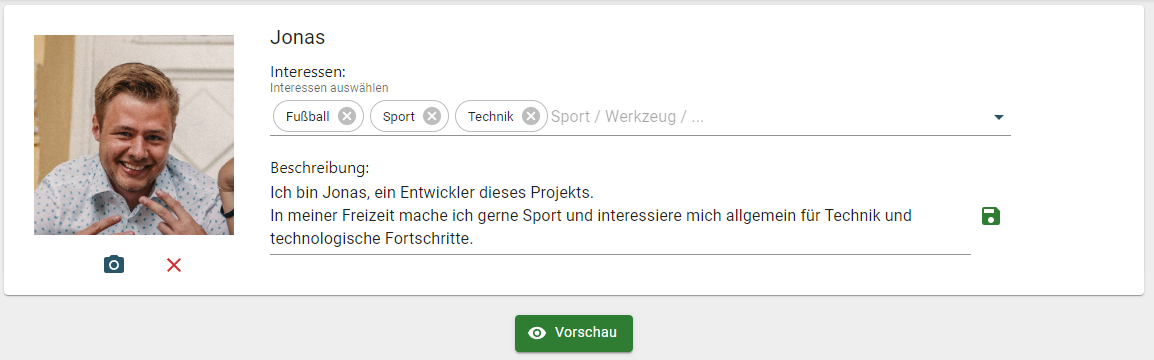
\includegraphics[width=1\textwidth]{figures/implementation/my-profile-header.png}
    \caption{Persönliches Profil}
    \label{fig:myProfileHeader}
  \end{centering}
\end{figure}

\subsection{Blockierte Nutzer}
\label{sec:blockedusers}

Um die Privatsphäre der Nutzer zu schützen, können diese andere Nutzer blockieren.
Blockierte Nutzer können dann nicht mehr auf das Profil des Blockierenden zugreifen und auch keine Nachrichten mehr schreiben.

Über die Profilseite kann ein Nutzer einen anderen Nutzer blockieren.

\begin{figure}[ht!]
  \begin{centering}
    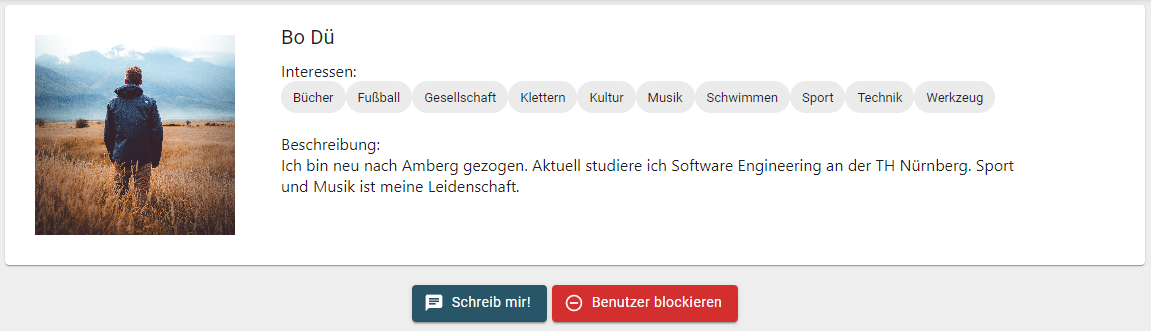
\includegraphics[width=1\textwidth]{figures/implementation/profile-header.png}
    \caption{Blockieren eines Nutzers}
    \label{fig:blockUser}
  \end{centering}
\end{figure}

Blockierte Nutzer kann man dann in der Anwendung unter dem Menüpunkt \textit{Blockiert} einsehen.
Dort wird jeder Nutzer oder Verein aufgeführt, welcher blockiert ist.
Mit einem Klick auf das „X“ wird der Block aufgehoben.

\begin{figure}[ht!]
  \begin{centering}
    
\includegraphics[width=.5\textwidth]{figures/implementation/blocked.png}
    \caption{Blockierte Nutzer}
    \label{fig:blocked}
  \end{centering}
\end{figure}

\section{Beiträge}
\label{sec:contributions}

Beiträge sind ein anderes wichtiges Feature von „Digital Dahoam“.
Hiermit können Nutzer Informationen austauschen, die für andere Nutzer interessant sein könnten.
Beiträge können von allen Nutzern erstellt werden, die sich registriert haben.
Es gibt folgende Typen von Beiträgen:

\begin{itemize}
  \item \textbf{Anfrage}: Hier können Nutzer eine Anfrage stellen, die dann von anderen Nutzern beantwortet werden kann. Anfragen können auch benutzt werden, wenn bestimmte Gegenstände im Haushalt fehlen, z. B. ein bestimmtes Werkzeug oder ein bestimmtes Lebensmittel.
  \item \textbf{Angebot}: Hier können Nutzer ein Angebot erstellen, das dann von anderen Nutzern angenommen werden kann. Dies kann wie Ebay-Kleinanzeigen benutzt werden, um überflüssige Gegenstände zu verkaufen.
  \item \textbf{Information}: Hier können Nutzer Informationen teilen, die für andere Nutzer interessant sein könnten.
  \item \textbf{Veranstaltung}: Hier können Nutzer Veranstaltungen erstellen, die dann von anderen Nutzern besucht werden können.
\end{itemize}

\subsection{Beiträge erstellen}
\label{sec:createpost}

Beiträge können mit einem Klick auf den Button \textit{Beiträge erstellen} erstellt werden.
Hier öffnet sich ein Pop-up, welchem der Nutzer den Titel, die Beschreibung, den Beitragstyp und die Kategorie des Beitrags eingeben kann.
Außerdem werden für jeden Beitrag das Startdatum, also ab wann der Beitrag gültig ist und angezeigt wird, und das Enddatum, also bis wann der Beitrag gültig ist und angezeigt wird, festgelegt.
Für Veranstaltungen gibt es zusätzlich noch den Ort und das Datum.
Sobald auf \textit{absenden} geklickt wird, wird der Beitrag in der Datenbank gespeichert und auf der Startseite angezeigt.

\begin{figure}[ht!]
  \begin{centering}
    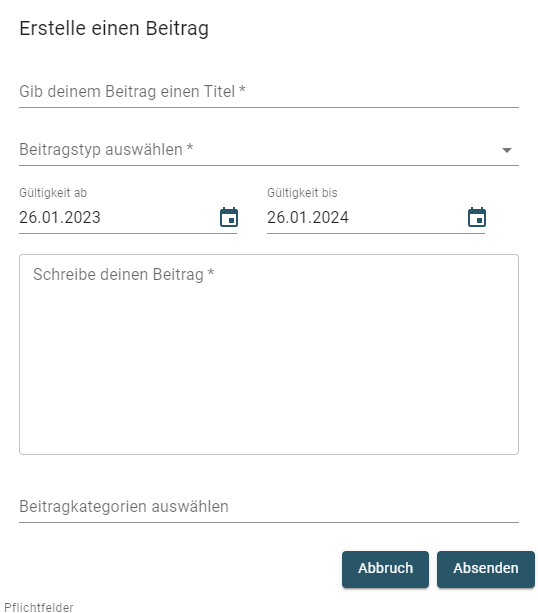
\includegraphics[width=.65\textwidth]{figures/implementation/createpost.png}
    \caption{Beiträge erstellen}
    \label{fig:createpost}
  \end{centering}
\end{figure}


\subsection{Alle Beiträge}
\label{sec:allposts}

Unter \textit{Alle Beiträge} findet man alle Beiträge, die ein valides Gültigkeitsdatum haben. Diese werden mit Titel, Beschreibung, Kategorie und Beitragstyp angezeigt.
Für Veranstaltungen gibt es zusätzlich noch den Ort und das Datum.

\begin{figure}[ht!]
  \begin{centering}
    
\includegraphics[width=.8\textwidth]{figures/implementation/beitrag.png}
    \caption{Beitrag}
    \label{fig:beitrag}
  \end{centering}
\end{figure}

Ein Problem, was es während der Implementierung zu lösen galt, war die richtige Filterung der Beiträge. Die hier verwendete Sortierfunktion (siehe \ref{code:filterPosts}) wurde dann für die restlichen Listen verwendet und die gefilterten Beiträge dort nur noch verfeinert.
Diese musste folgendes erfüllen:

\begin{itemize}
  \item Eigene Beiträge werden immer angezeigt.
  \item Beiträge, die nicht mehr gültig sind, werden nicht angezeigt.
  \item Beiträge von blockierten Nutzern werden nicht angezeigt.
  \item Beiträge müssen nach Datum sortiert werden.
\end{itemize}

Mit dem Klick auf die 3 kleinen Punkte in der rechten oberen Ecke öffnet man das Beitragsmenü. Hier gibt es folgende Punkte:

\begin{itemize}
  \item \textbf{Beitrag zum Merkzettel}: Hinzufügen eines Inhalts zum Merkzettel.
  \item \textbf{Details}: Anzeigen der Details des Beitrags. (siehe \ref{fig:details})
  \item \textbf{Zum Autor}: Direkter Link zum Profil des Autors.
  \item \textbf{Nachricht an Autor}: Direkter Link zur Nachrichtenfunktion, um dem Autor eine Nachricht zu schicken.
\end{itemize}

\begin{figure}[ht!]
  \begin{centering}
    \includegraphics[width=.25\textwidth]{figures/implementation/beitragsmenü.png}
    \caption{Beitragsmenü}
    \label{fig:beitragsmenü}
  \end{centering}
\end{figure}

\clearpage
\subsection{Profilseite}
\label{sec:profilepage}

Auf der Profilseite kann der Nutzer werden seine Beiträge angezeigt.
Hier werden auch abgelaufene Beiträge angezeigt und grau hinterlegt.

\begin{figure}[ht!]
  \begin{centering}
    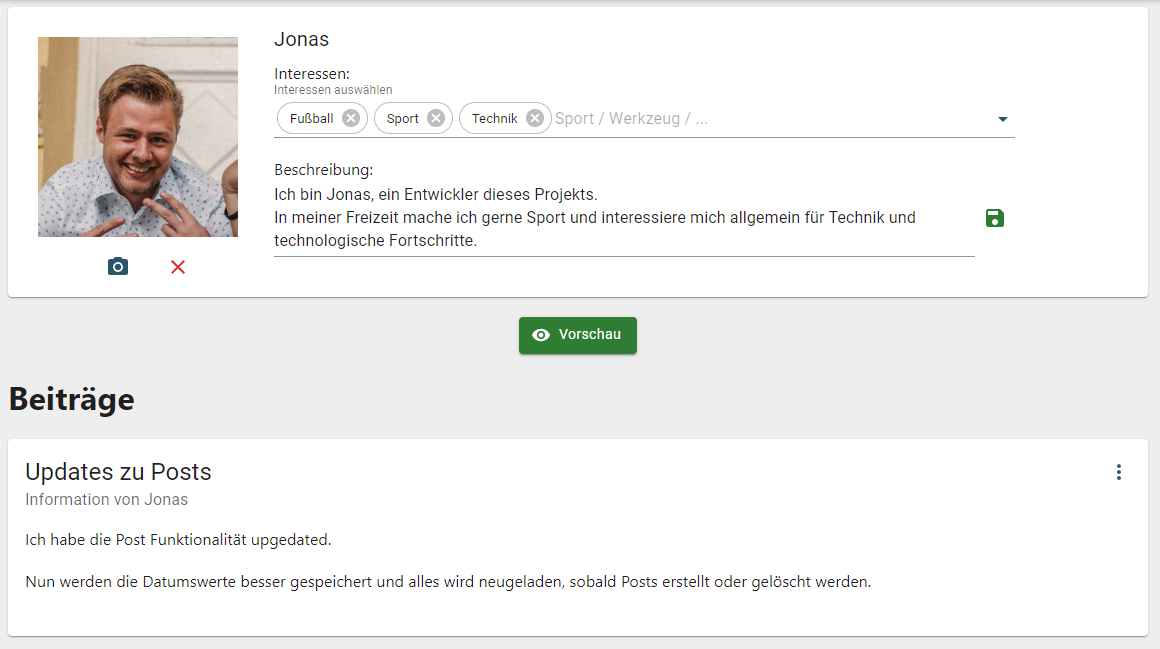
\includegraphics[width=1\textwidth]{figures/implementation/userposts.png}
    \caption{Beiträge des Nutzers}
    \label{fig:userposts}
  \end{centering}
\end{figure}

\subsection{Merkzettel}
\label{sec:bookmark}

Beiträge, die für den Merkzettel markiert sind erscheinen dort, und können dort auch wieder entfernt werden.
Außerdem werden sie nach Beitragstyp gruppiert.

\begin{figure}[ht!]
  \begin{centering}
    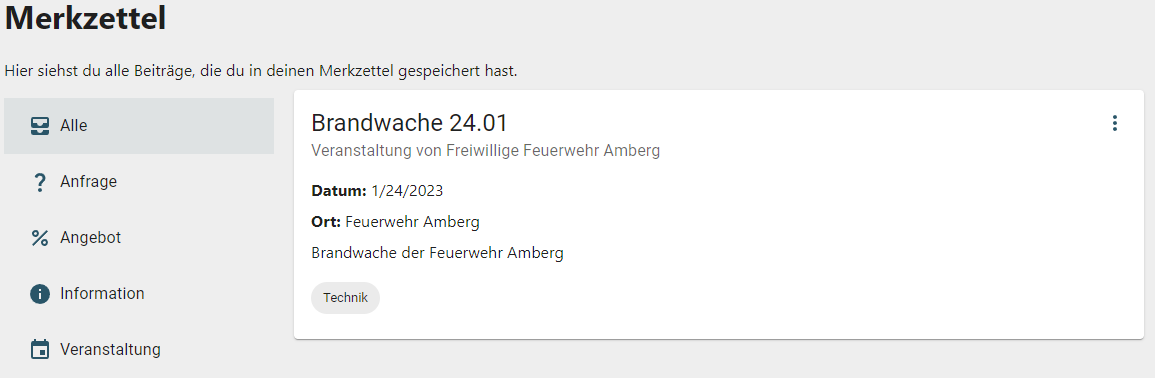
\includegraphics[width=1\textwidth]{figures/implementation/merkzettel.png}
    \caption{Merkzettel}
    \label{fig:merkzettel}
  \end{centering}
\end{figure}

\clearpage
\subsection{Marktplatz}
\label{sec:marketplace}

Auf dem Marktplatz können Personen und Beiträge durchsucht werden.
Durch den Filter auf Kategorien, Informationen oder Veranstaltungen findet man schnell den richtigen Beitrag.

\begin{figure}[ht!]
  \begin{centering}
    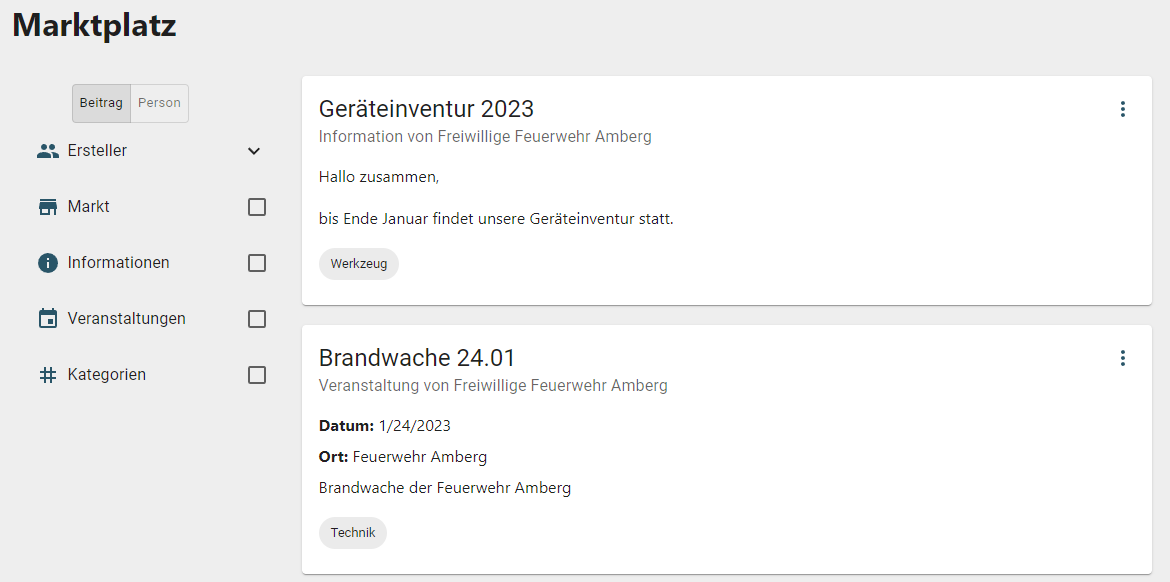
\includegraphics[width=1\textwidth]{figures/implementation/marktplatz.png}
    \caption{Marktplatz}
    \label{fig:marktplatz}
  \end{centering}
\end{figure}


\subsection{Dashboard}
\label{sec:dashboard}

Auf der Startseite werden aktuelle Beiträge aus der Nähe angezeigt, sowie die Veranstaltungen, die der Nutzer auf dem Merkzettel hat.

\begin{figure}[ht!]
  \begin{centering}
    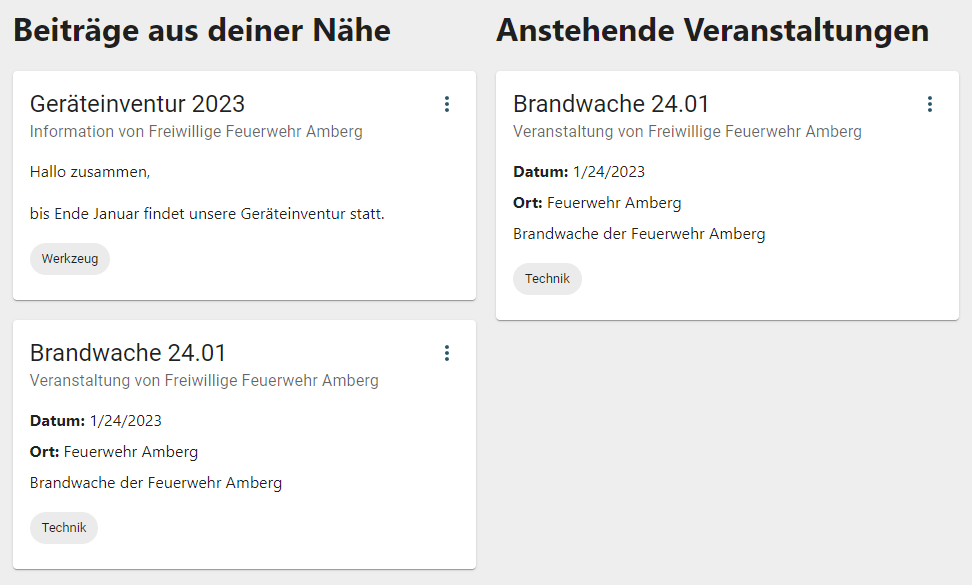
\includegraphics[width=.8\textwidth]{figures/implementation/dashboard.png}
    \caption{Dashboard}
    \label{fig:dashboard}
  \end{centering}
\end{figure}

% \include{content/07_sprints}
% \include{content/08_outlook}

\appendix
\pagenumbering{Alph}
\renewcommand{\thechapter}{\Alph{chapter}}
\renewcommand{\thesection}{\Roman{section}}
\renewcommand{\thesubsection}{\Roman{subsection}}
\renewcommand\floatpagefraction{0.1}
\clearpage
\chapter{Anhang}
\label{appendix:annex}

\section{Bilder}
\label{annex:images}

\begin{figure}[ht!]
  \begin{centering}
    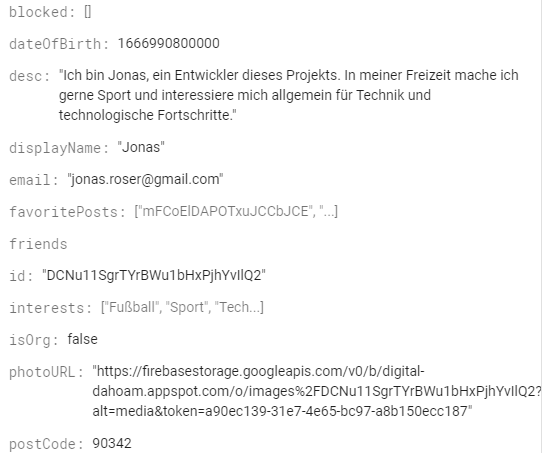
\includegraphics[width=1\textwidth]{figures/implementation/firestore-user.png}
    \caption{Benutzerdatensatz in Firestore}
    \label{fig:firestoreUser}
  \end{centering}
\end{figure}

\begin{figure}[ht!]
  \begin{centering}
    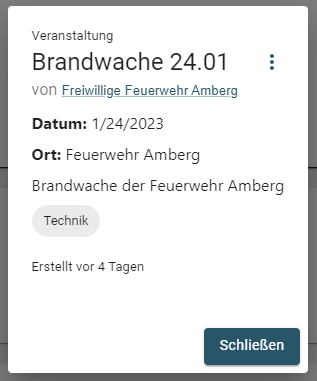
\includegraphics[width=.75\textwidth]{figures/implementation/details.png}
    \caption{Beitragsdetails}
    \label{fig:details}
  \end{centering}
\end{figure}

\clearpage
\section{Code}
\label{annex:code}

\begin{lstlisting}[language=JavaScript, label=code:filterPosts, title={Filterfunktion der Beiträge}]
const filtered = posts
.filter((post) => !currentUser?.blocked?.includes(post.author.id))
.filter((post) => {
  // check validity
  if (currentUser?.id === post.author.id) {
    return true
  }

  if (!(post.validityStart && post.validityEnd)) {
    // no validity set
    return true
  }
  console.log(
    moment(post.validityStart).toDate().getTime(),
    moment(post.validityStart).toDate().getTime() <= new Date().getTime(),
  )
  if (
    moment(post.validityStart).toDate().getTime() >= new Date().getTime() &&
    moment(post.validityEnd).toDate().getTime() <= new Date().getTime()
  ) {
    return true
  } else {
    return false
  }
})
\end{lstlisting}

\backmatter
\listoffigures
\listoftables
\bibliographystyle{IEEEtran}
\bibliography{refs}

\end{document}
